\documentclass{article}
%\documentclass[journal,transmag]{IEEEtran}
%\documentclass[10pt, conference]{IEEEtran}
\usepackage{amsmath}
\usepackage{graphicx}
%\usepackage{listings}
%\usepackage{circuitikz}
\usepackage{lscape}
\usepackage{ulem}
\usepackage{float}


\usepackage[scale=0.8]{geometry}
\begin{document}

\title{E6312: Problem Set 2}
\author{Miles Sherman}
\date{\today}
\maketitle

%\textit{The previous homework sets have led me through the investigation of single transistor behaviors and basic amplifier circuits. In this problem set, I examine the use of basic and intermediate biasing circuits. In addition, I begin work with basic differential stages.}

\section{Problem 1}
\subsection{}
\begin{figure}[H]
\centering
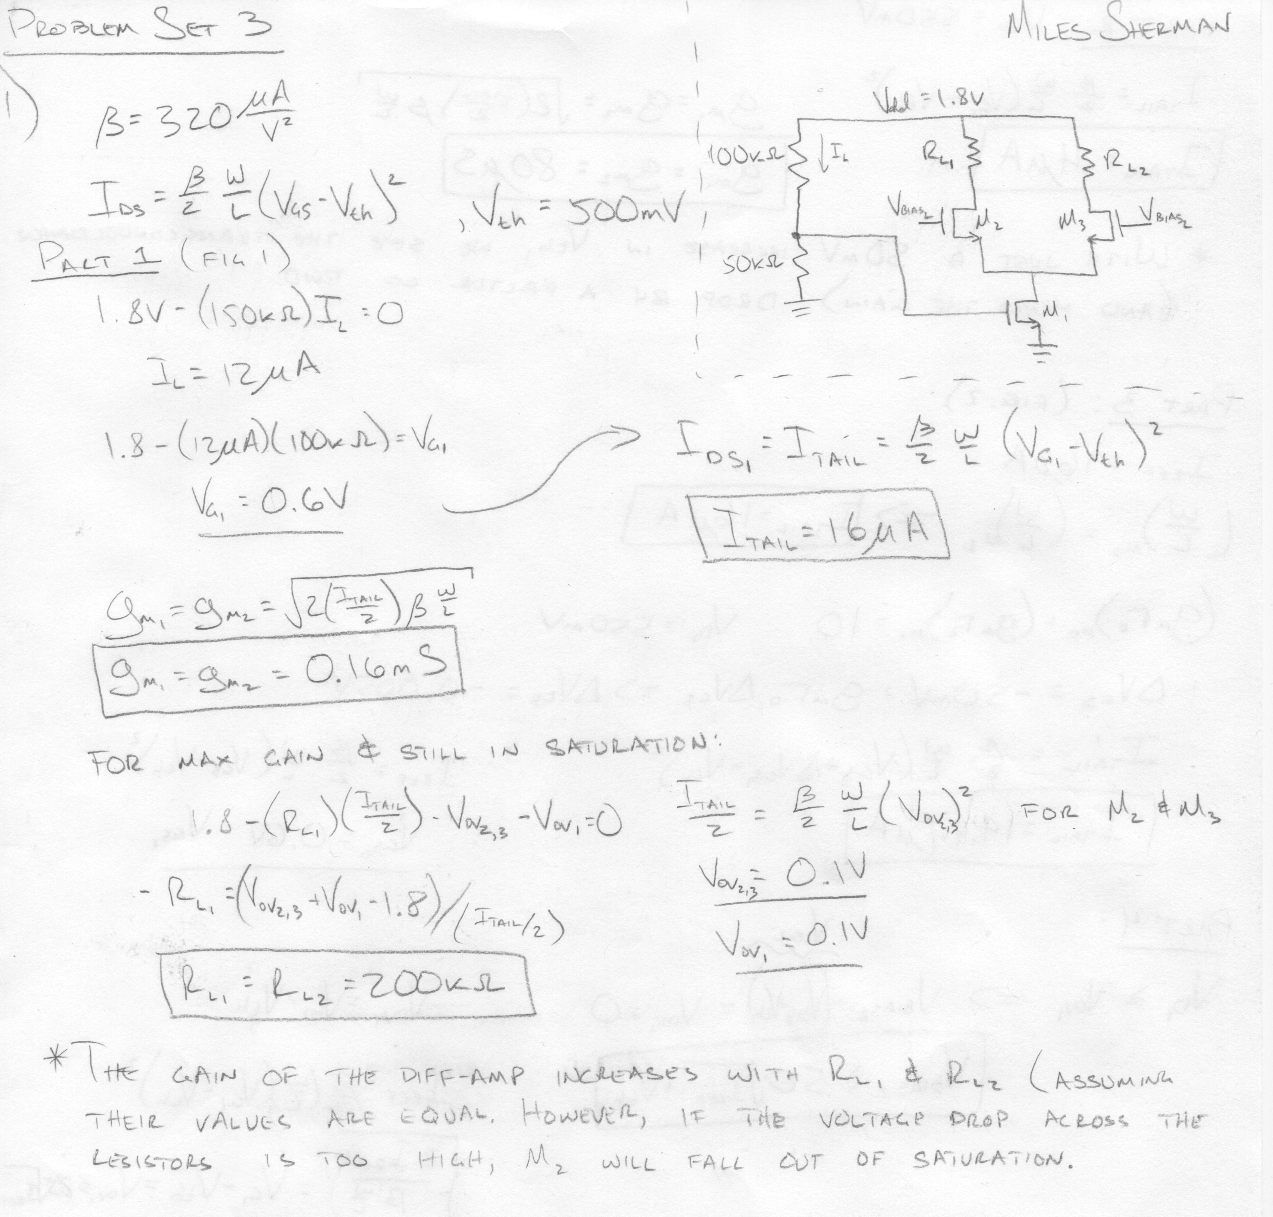
\includegraphics[width=6in]{1_1}
\caption{Hand-Written Work for Problem 1.1}
\label{1_1}
\end{figure}

\subsection{}
\begin{figure}[H]
\centering
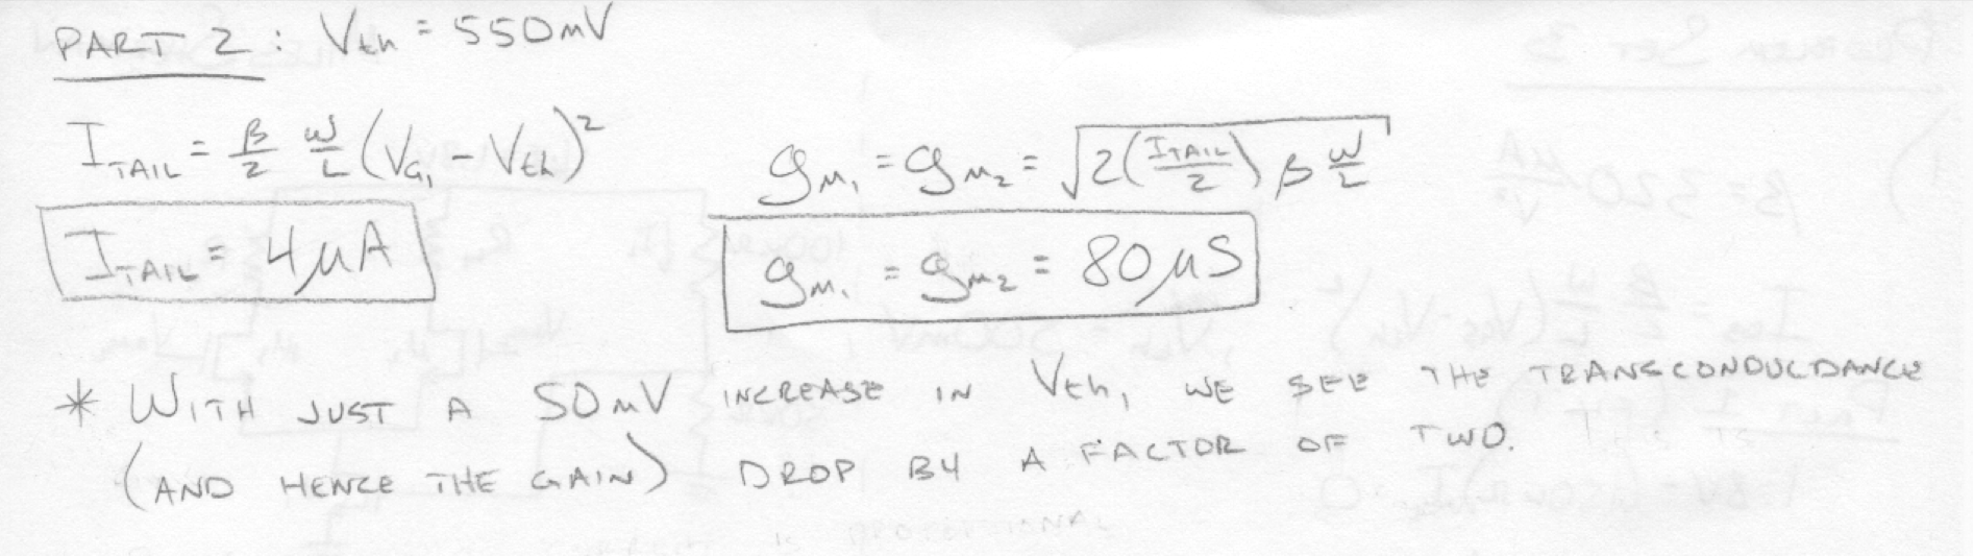
\includegraphics[width=6in]{1_2a.pdf}
\caption{Hand-Written Work for Problem 1.2}
\label{1_2}
\end{figure}

\subsection{}
\begin{figure}[H]
\centering
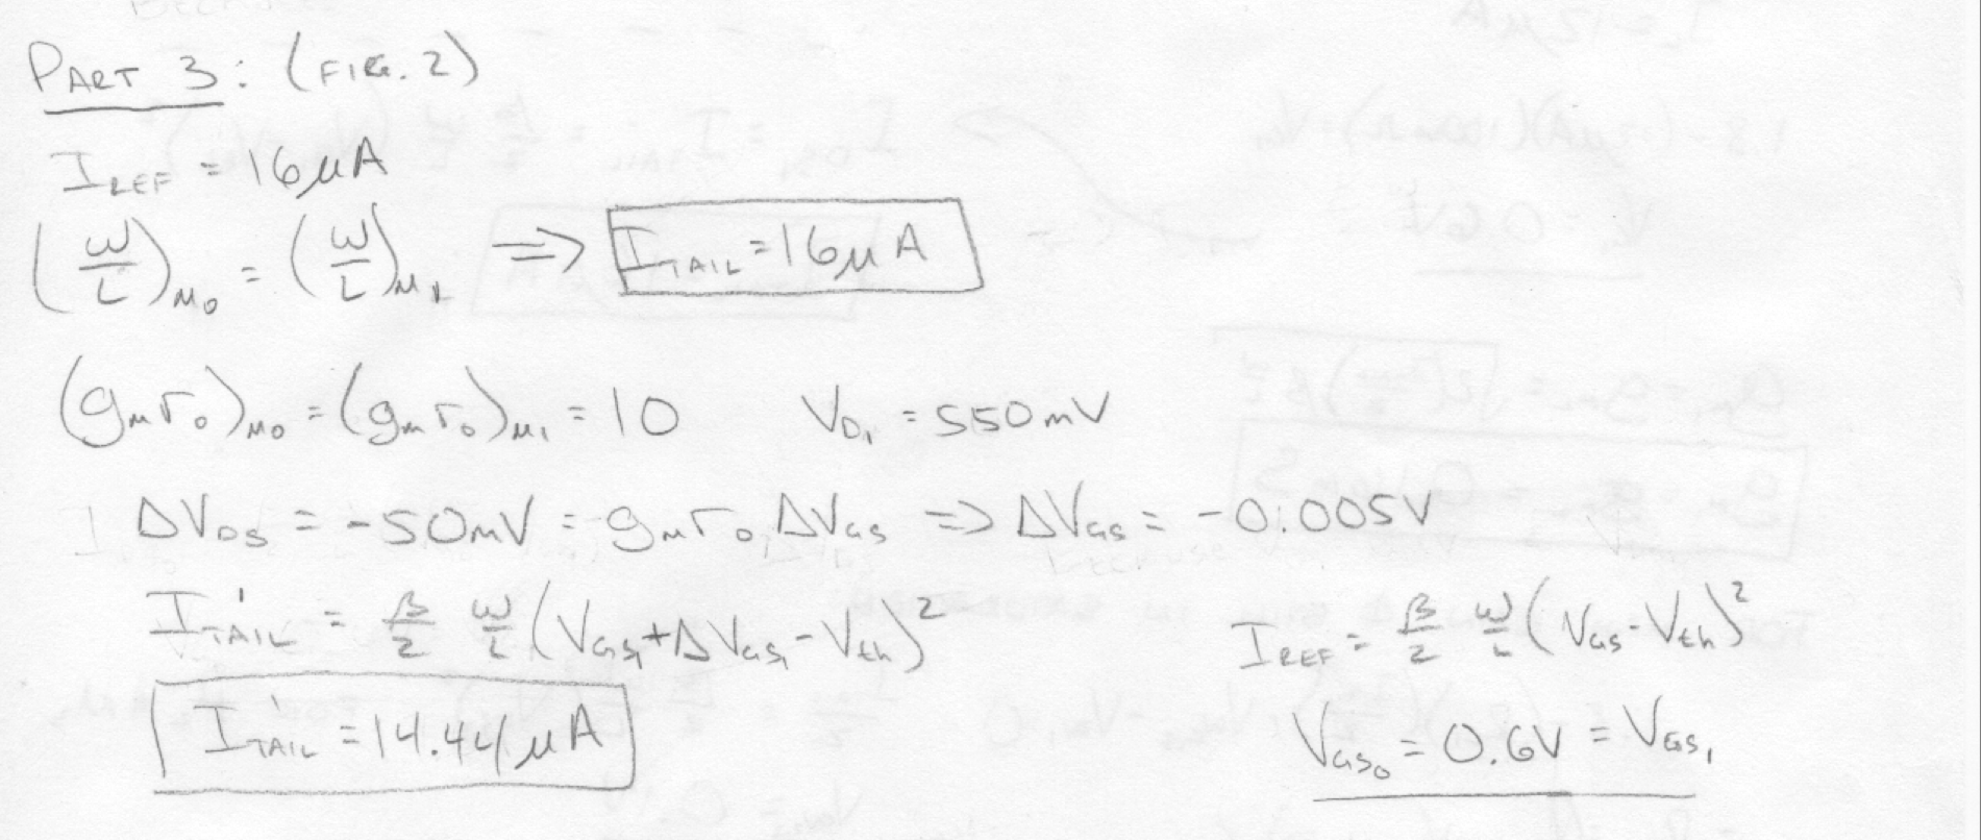
\includegraphics[width=6in]{1_2b}
\caption{Hand-Written Work for Problem 1.3}
\label{1_3}
\end{figure}

\subsection{}
\begin{figure}[H]
\centering
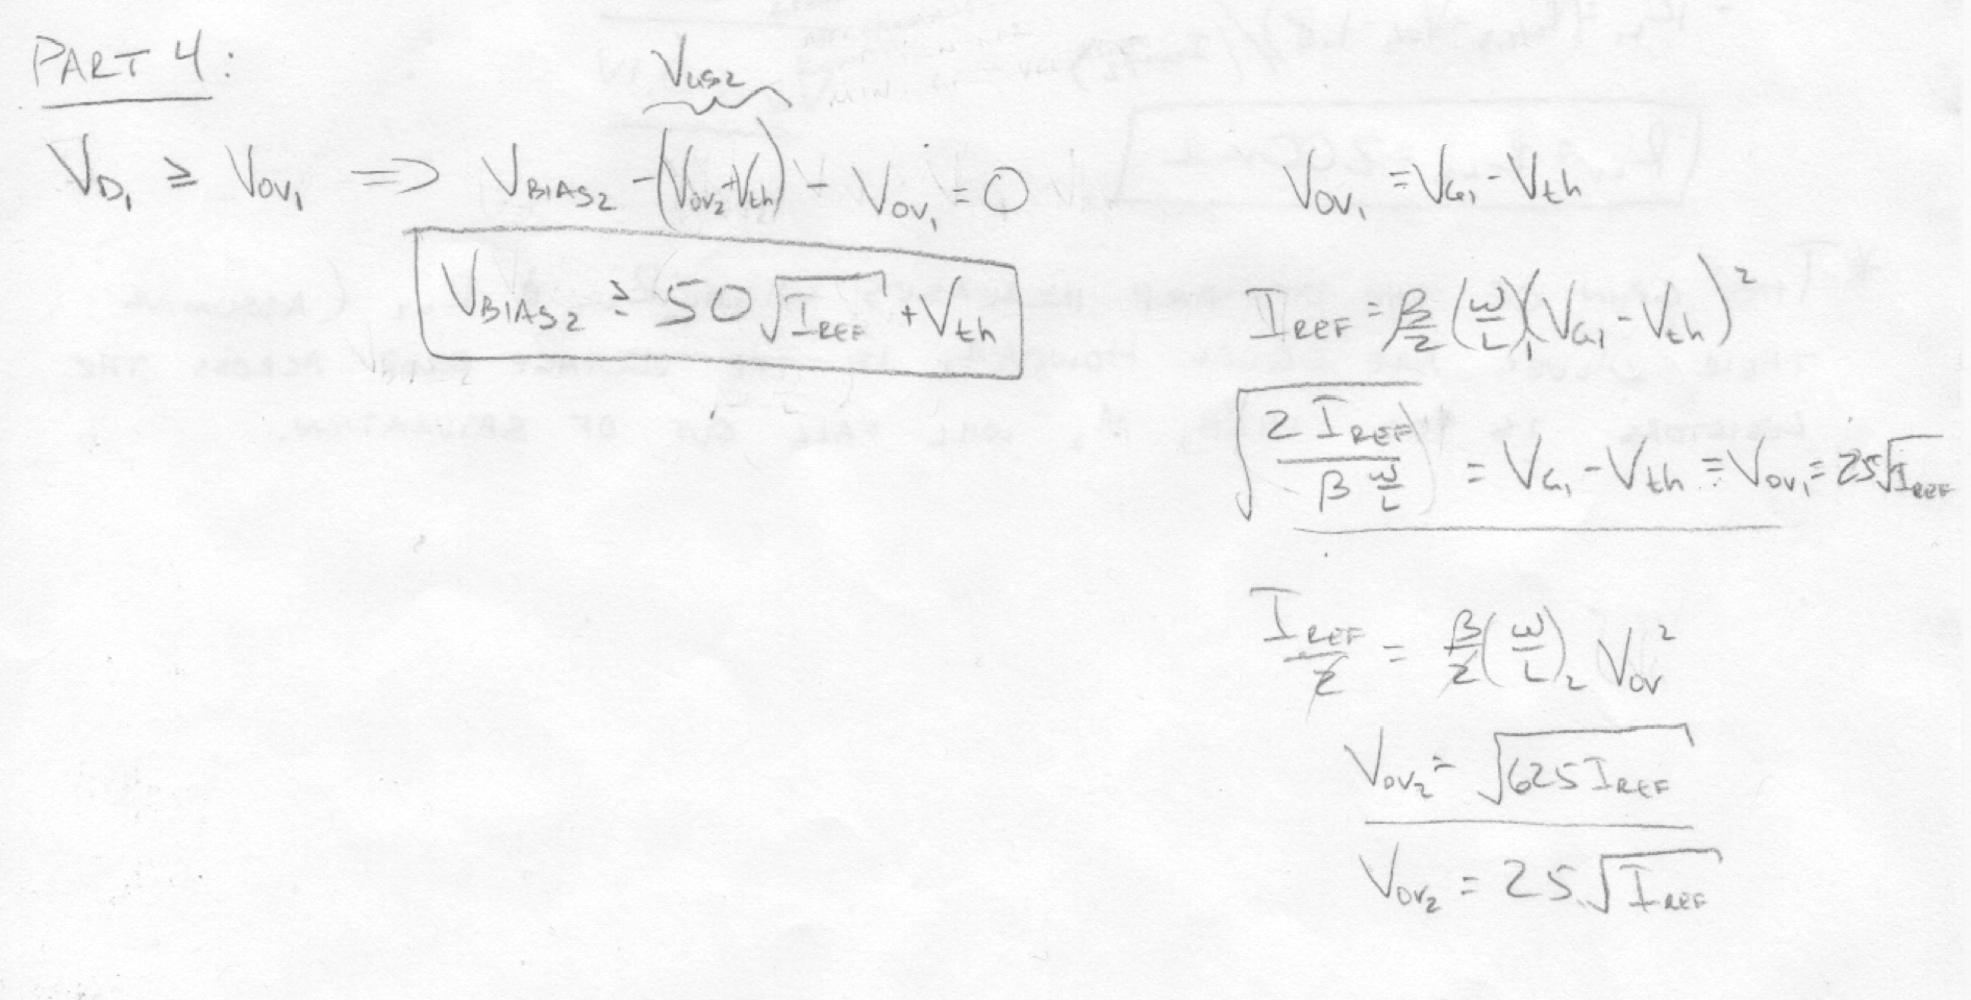
\includegraphics[width=6in]{1_2c}
\caption{Hand-Written Work for Problem 1.4}
\label{1_4}
\end{figure}

\begin{figure}[H]
\centering
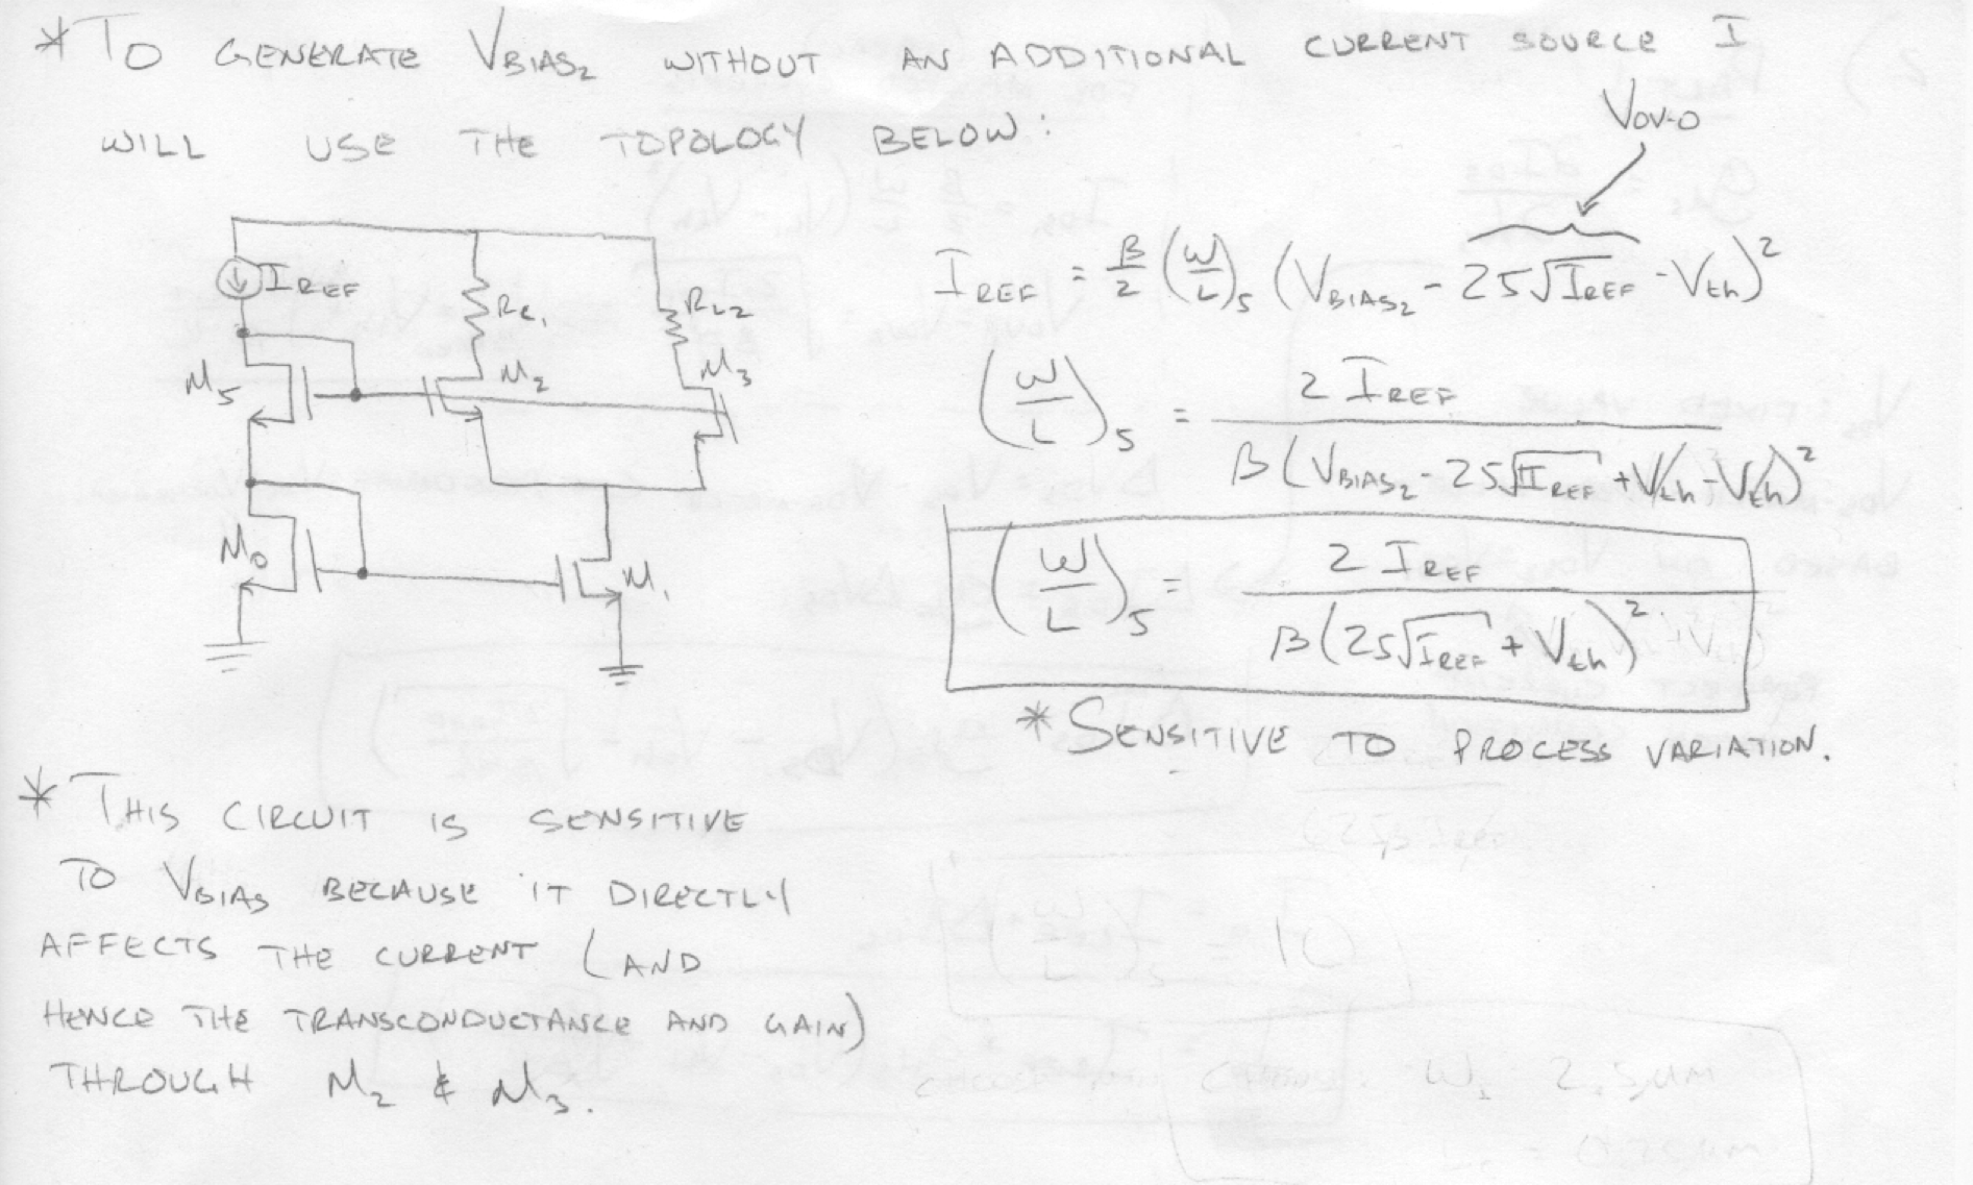
\includegraphics[width=6in]{1_3a}
\caption{Hand-Written Work for Problem 1.4 (ctnd)}
\label{1_4cntd}
\end{figure}

\subsection{(including additional credit problem)}
\begin{figure}[H]
\centering
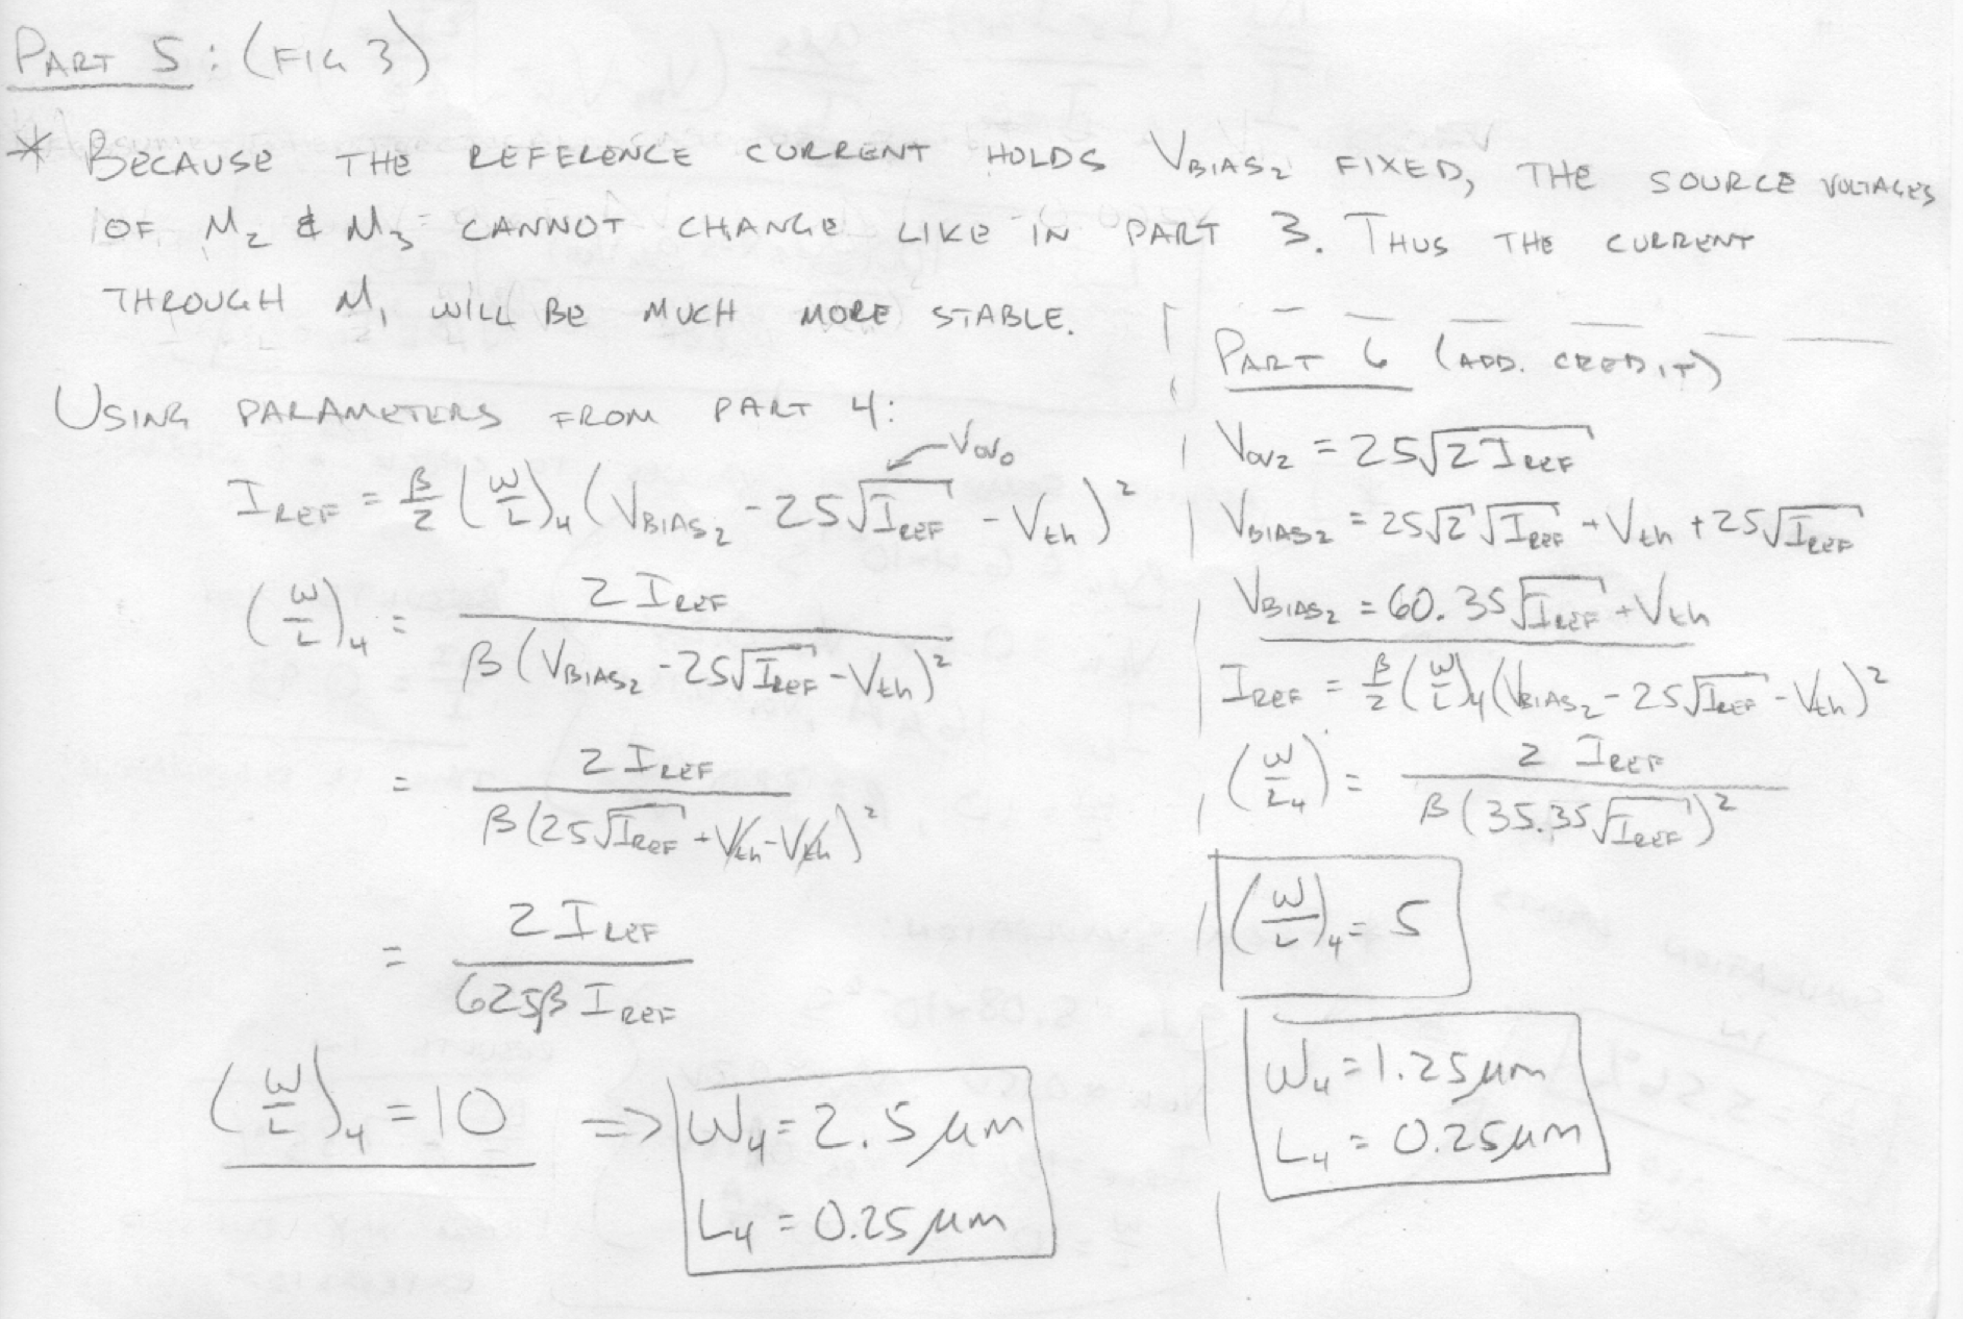
\includegraphics[width=6in]{1_3b}
\caption{Hand-Written Work for Problem 1.5}
\label{1_5}
\end{figure}
\newpage

\section{Problem 2}
\subsection{}
For this problem, I performed hand-written calculations and verified my calculations with simulations (see Figures \ref{2_1_schem} and \ref{2_1_dcop}). It should be noted that while my calculated values were not identical to those from simulations, they were reasonably close considering the assumptions made. These assumptions include $\beta = 320\frac{\mu A}{V^2}$ and $V_{th} = 500mV$.

\begin{figure}[H]
\centering
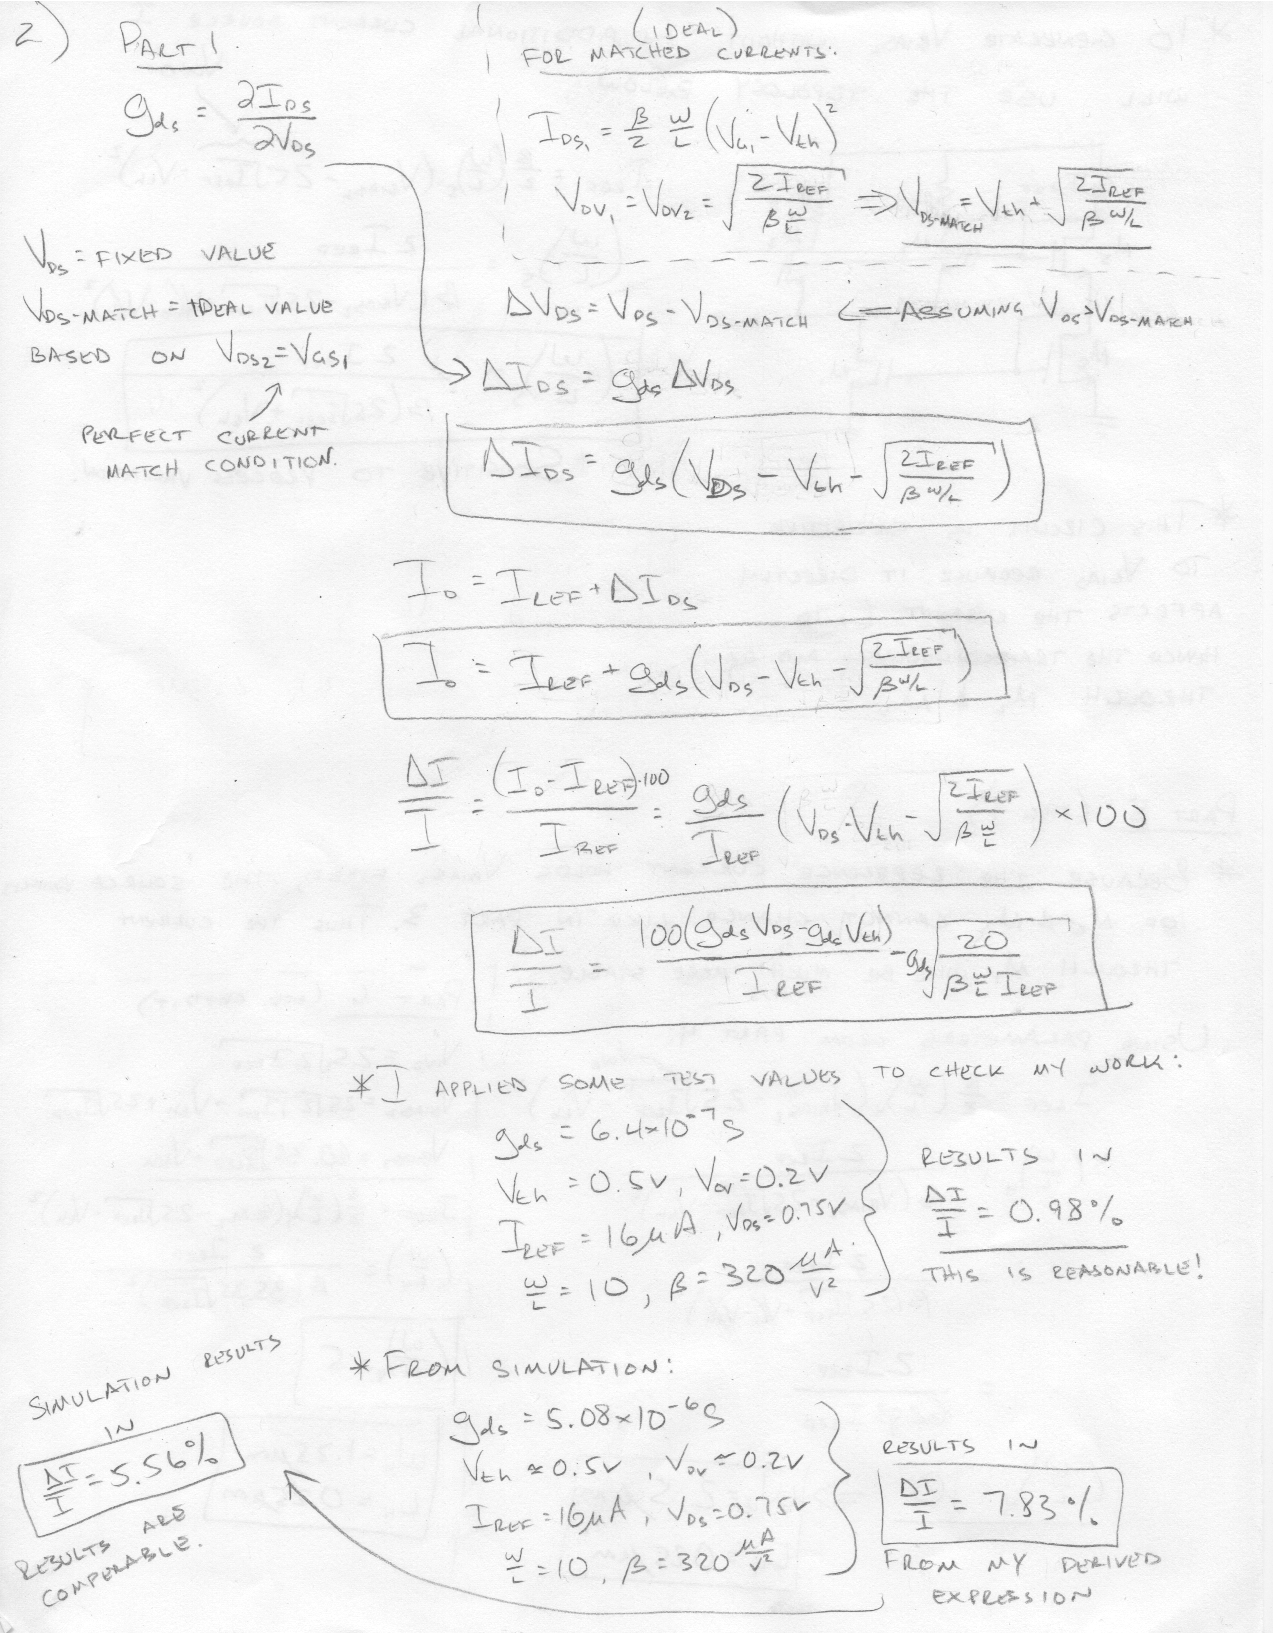
\includegraphics[width=6in]{1_4}
\caption{Hand-Written Work for Problem 2.1}
\label{2_1}
\end{figure}

\begin{figure}[H]
\centering
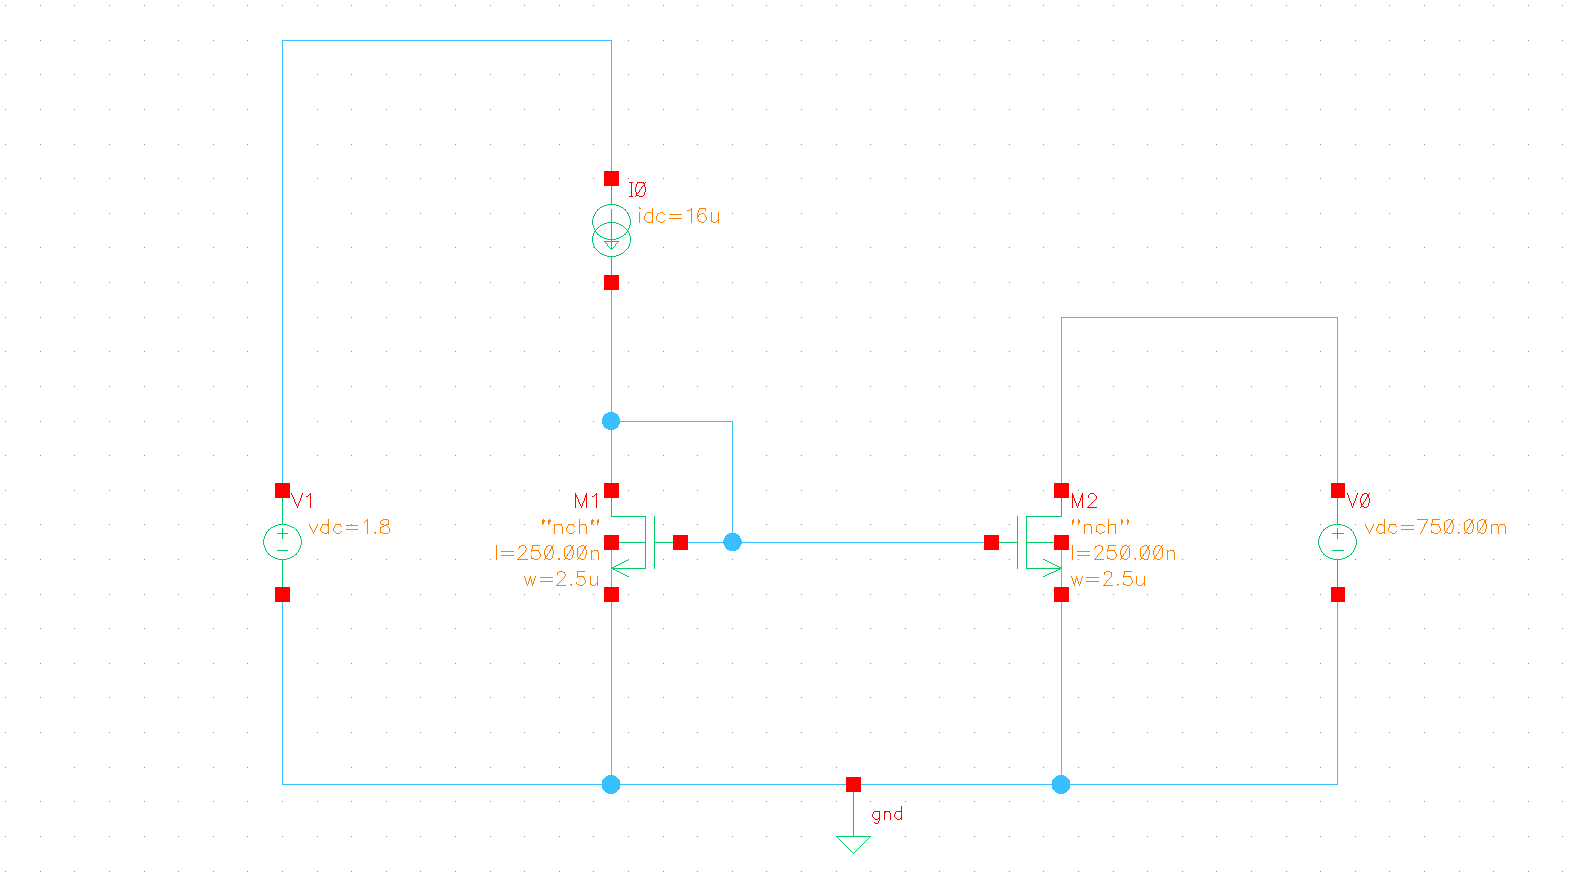
\includegraphics[width=6in]{p2_1_schem.png}
\caption{Schematic to Verify Sizing Calculations}
\label{2_1_schem}
\end{figure}

\begin{figure}[H]
\centering
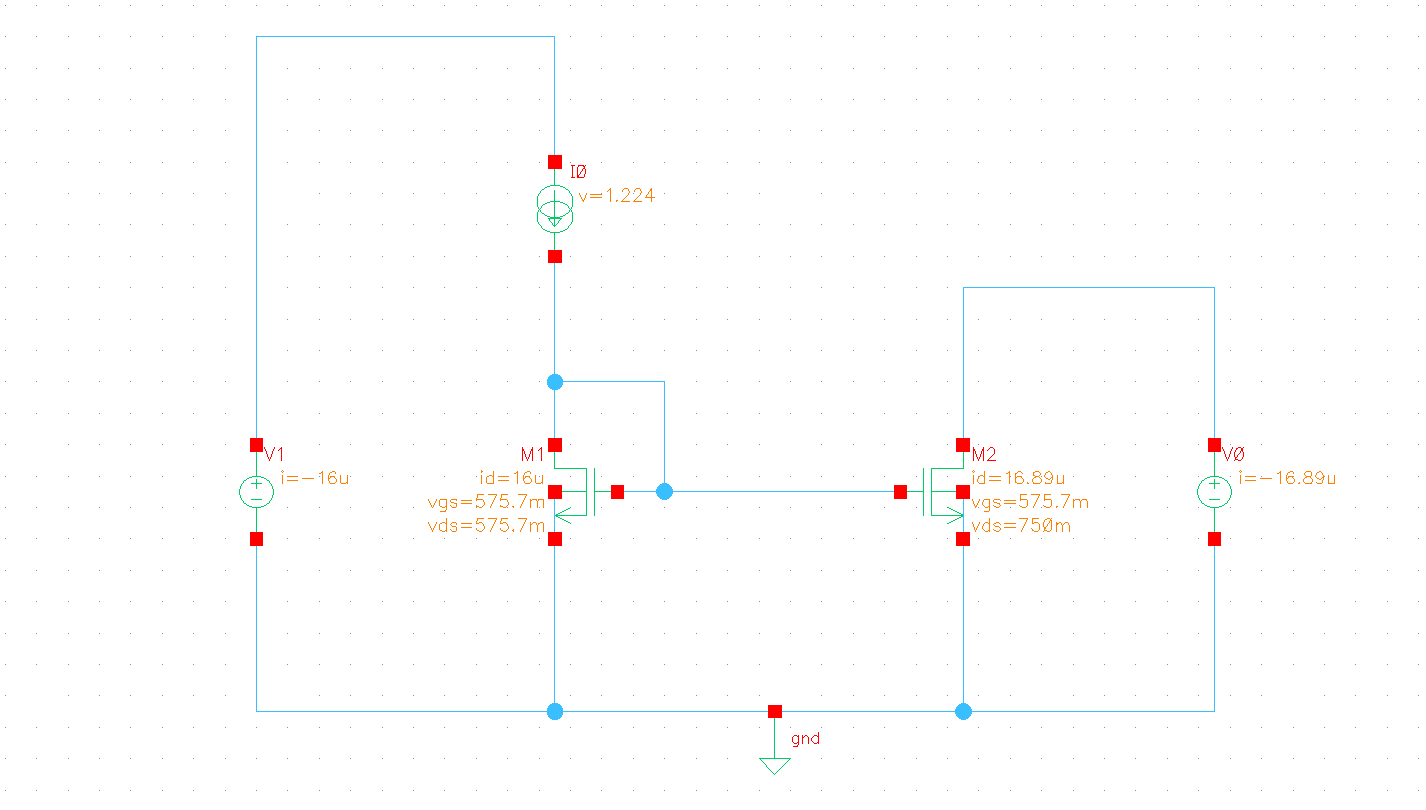
\includegraphics[width=6in]{p2_1_dcop.png}
\caption{Schematic with DC Operating Point Annotations To Verify Calculations}
\label{2_1_dcop}
\end{figure}
\newpage

\subsection{}
For this problem, I performed hand-written calculations and verified my calculations with simulations (see Figures \ref{2_2_schem}, \ref{2_2_dcop}, \ref{2_2_10p_schem}, and \ref{2_2_10p_dcop}). Again because I made assumptions in my hand calculations, I had to slightly modify my size values in simulation to attain the correct current error. However, it was still very necessary to perform the calculations before simulating because they streamlined the design process. Without my calculations to determine at least a ballpark for each component parameter, the design would have been much more difficult and confusing.

\begin{figure}[H]
\centering
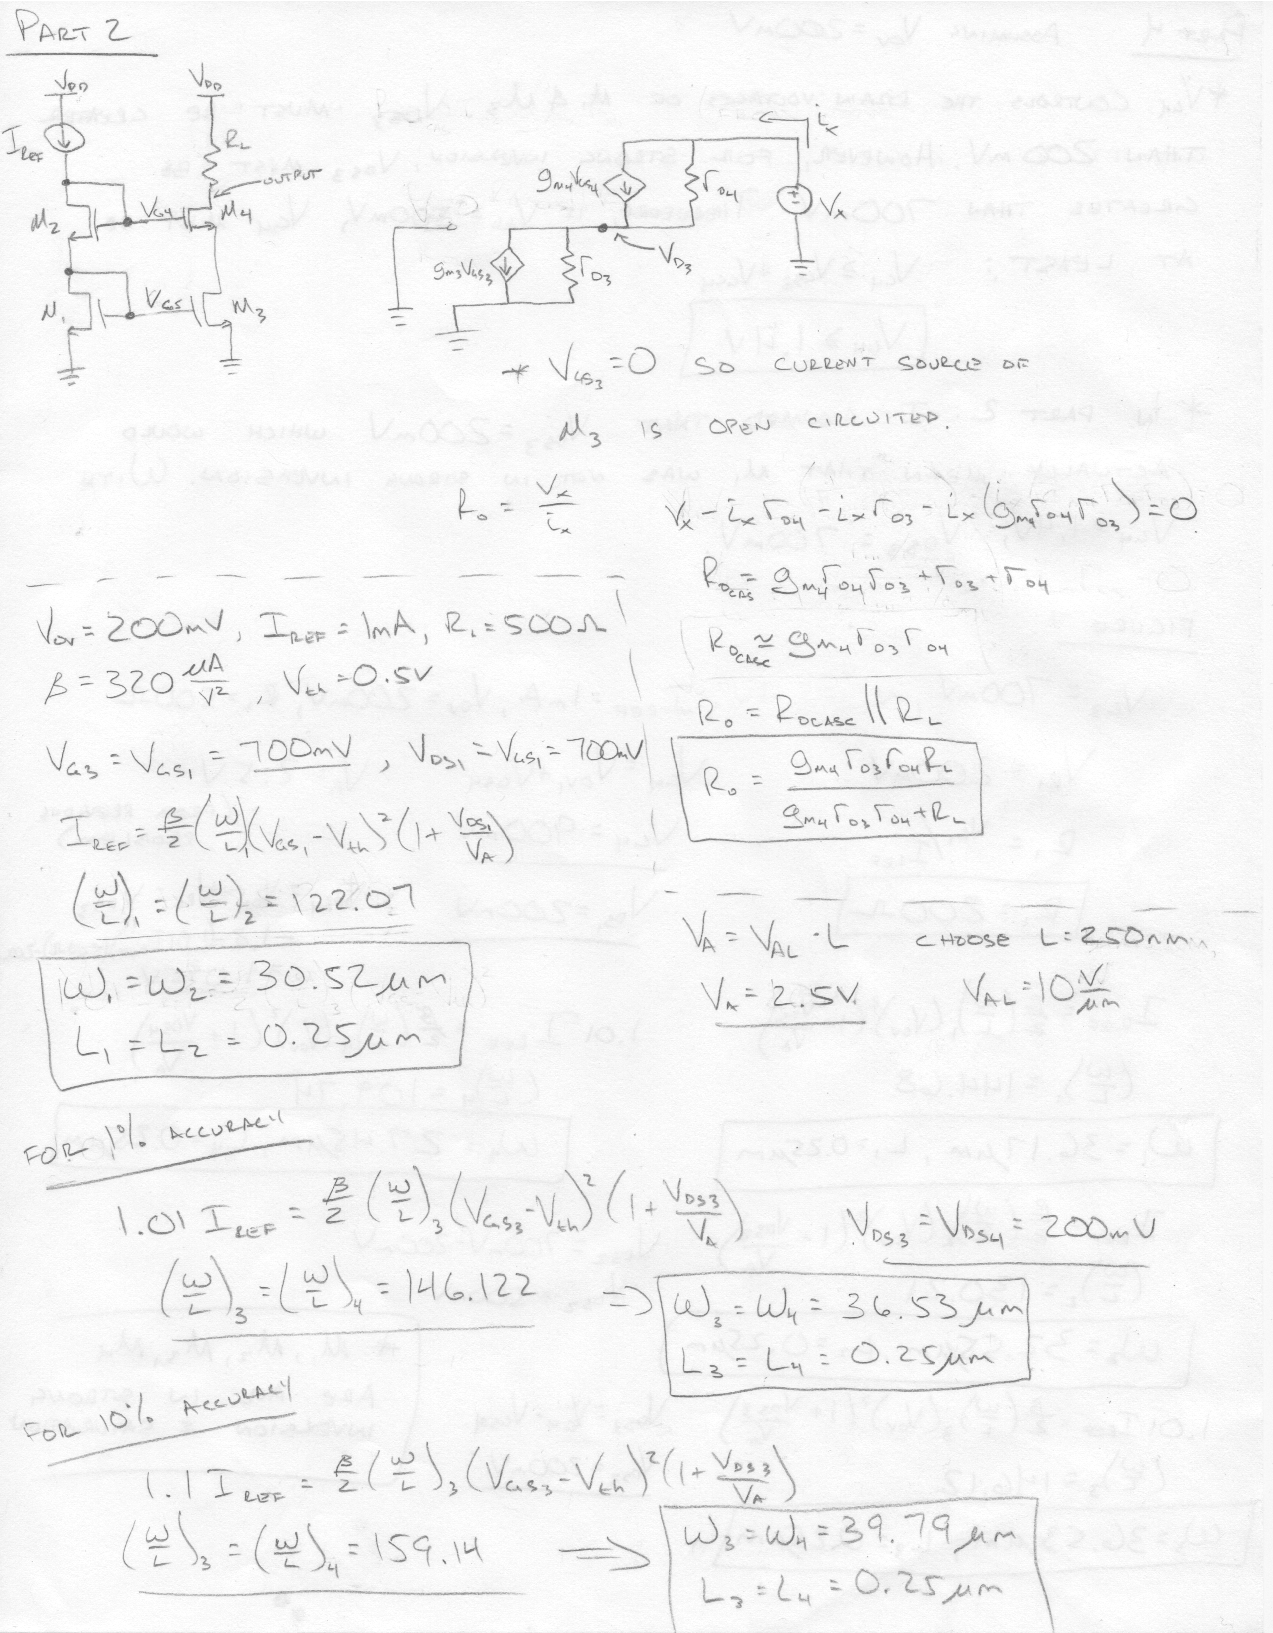
\includegraphics[width=6in]{1_5}
\caption{Hand-Written Work for Problem 2.1}
\label{2_1}
\end{figure}

\begin{figure}[H]
\centering
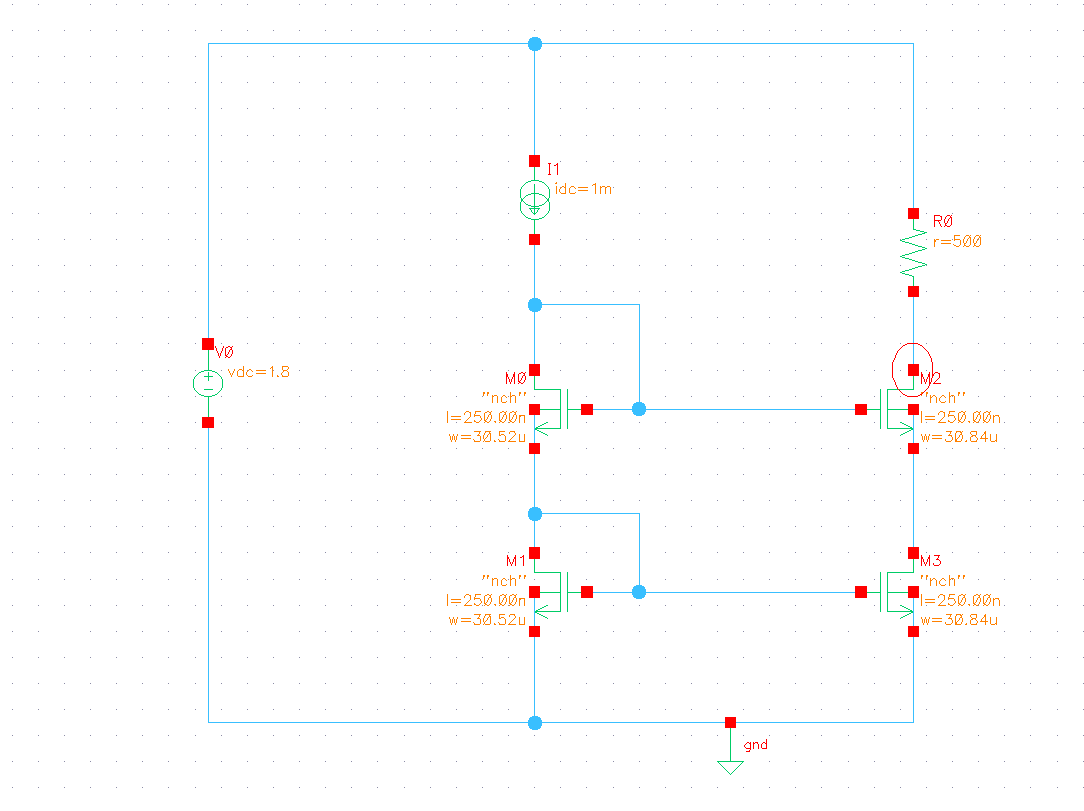
\includegraphics[width=6in]{p2_2_schem_1p.png}
\caption{Schematic to Verify Sizing Calculations for 1\% Current Error}
\label{2_2_schem}
\end{figure}

\begin{figure}[H]
\centering
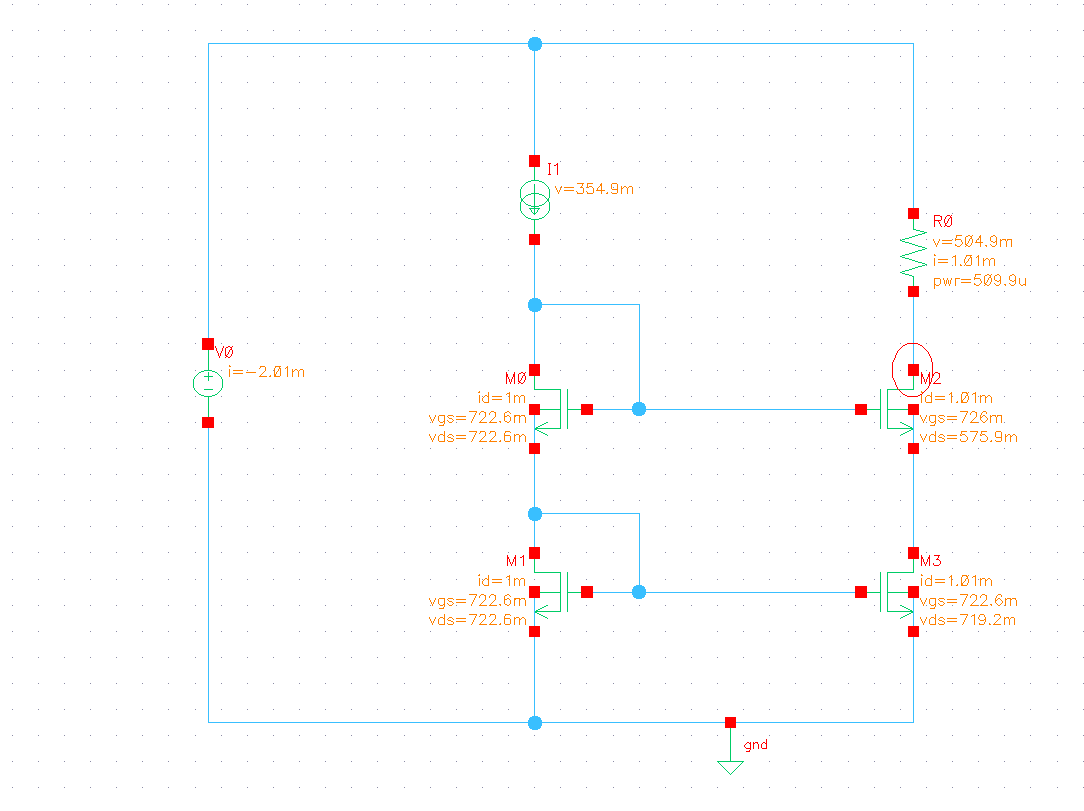
\includegraphics[width=6in]{p2_2_dcop_1p.png}
\caption{Schematic with DC Operating Point Annotations Verifying Sizing Calculations for 1\% Current Error}
\label{2_2_dcop}
\end{figure}

\begin{figure}[H]
\centering
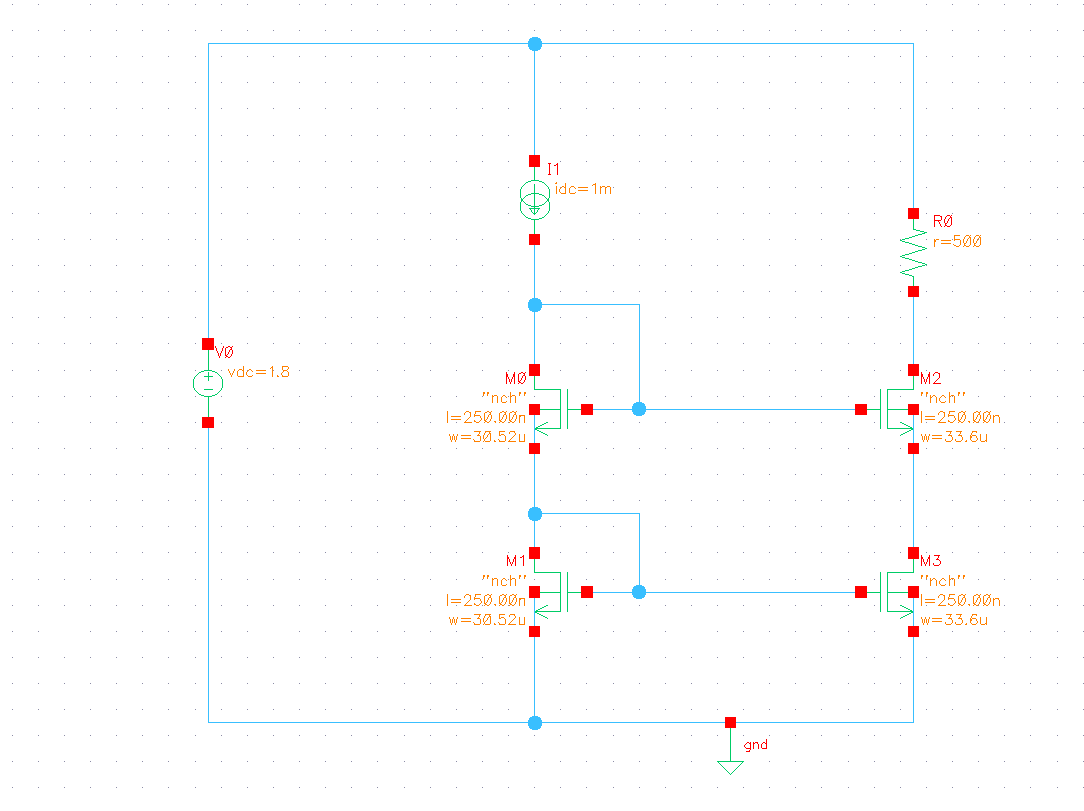
\includegraphics[width=6in]{p2_2_schem.png}
\caption{Schematic to Verify Sizing Calculations for 10\% Current Error}
\label{2_2_10p_schem}
\end{figure}


\begin{figure}[H]
\centering
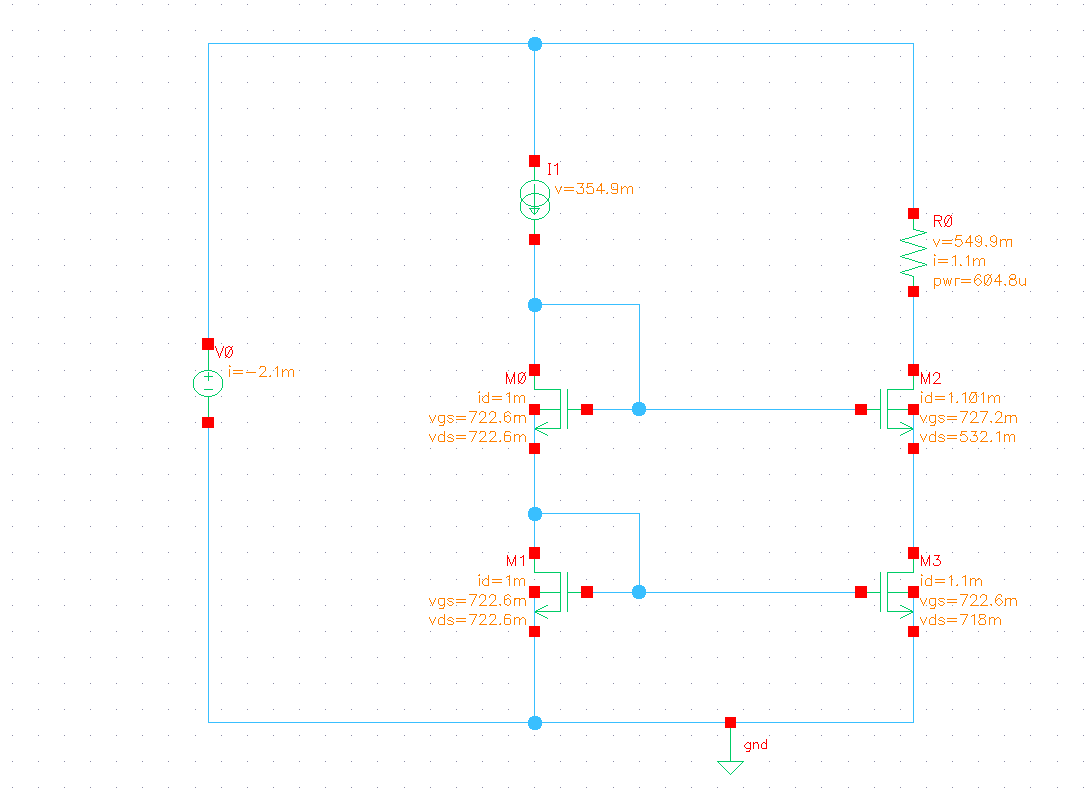
\includegraphics[width=6in]{p2_2_dcop.png}
\caption{Schematic with DC Operating Point Annotations Verifying Sizing Calculations for 10\% Current Error}
\label{2_2_10p_dcop}
\end{figure}
\newpage

\subsection{}
For this problem, I simulated current against Drain Voltage to show how the error trends. For Figure 5 from the from the original assignment write-up, I swept $V_{DS}$ and the current error is shown in Figure \ref{2_3a}. In this plot, the current error is somewhat consistent for most voltage values but drops off around 200mV. This voltage is the compliance of this circuit because it is the minimum voltage to keep M2 in saturation.

For Figure 6 from the original assignment write-up, I swept the drain voltage of M4 using a voltage source and this time the current is seen to saturate around 400mV (the minimum voltage to keep both M3 and M4 in saturation). This plot can be seen in Figure \ref{2_3b}.

\begin{figure}[H]
\centering
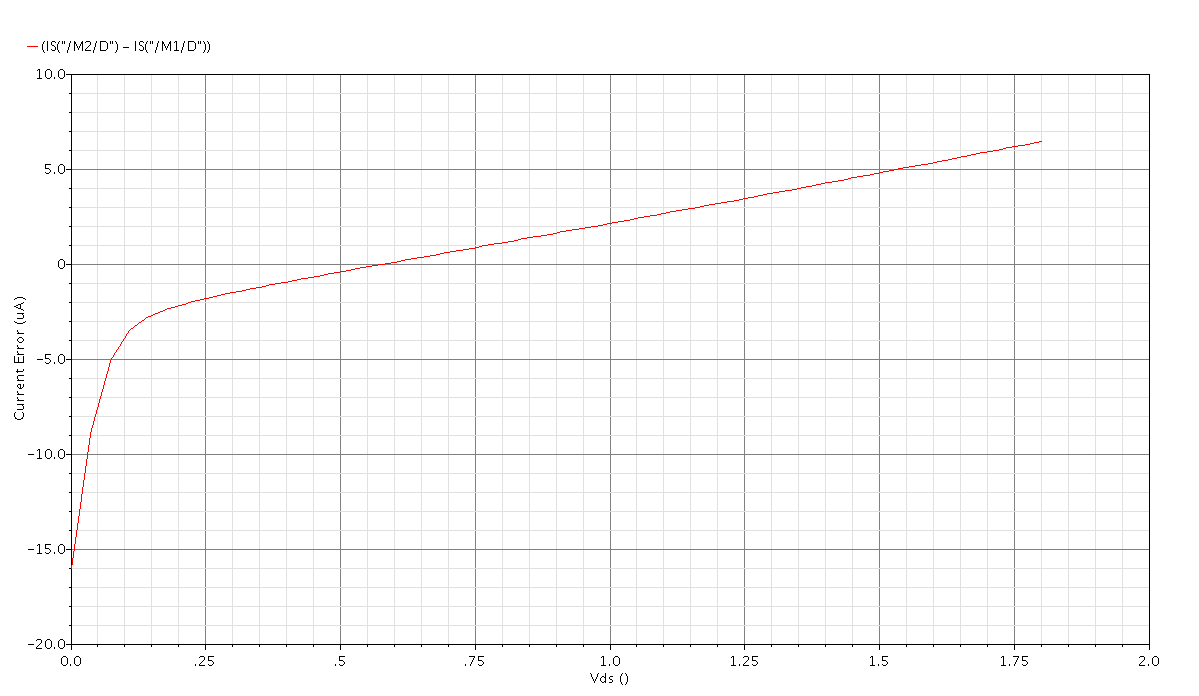
\includegraphics[width=6in]{p2_3_1}
\caption{Current Gain vs. $V_{DS}$ for the Basic Current Mirror Configuration}
\label{2_3a}
\end{figure}

\begin{figure}[H]
\centering
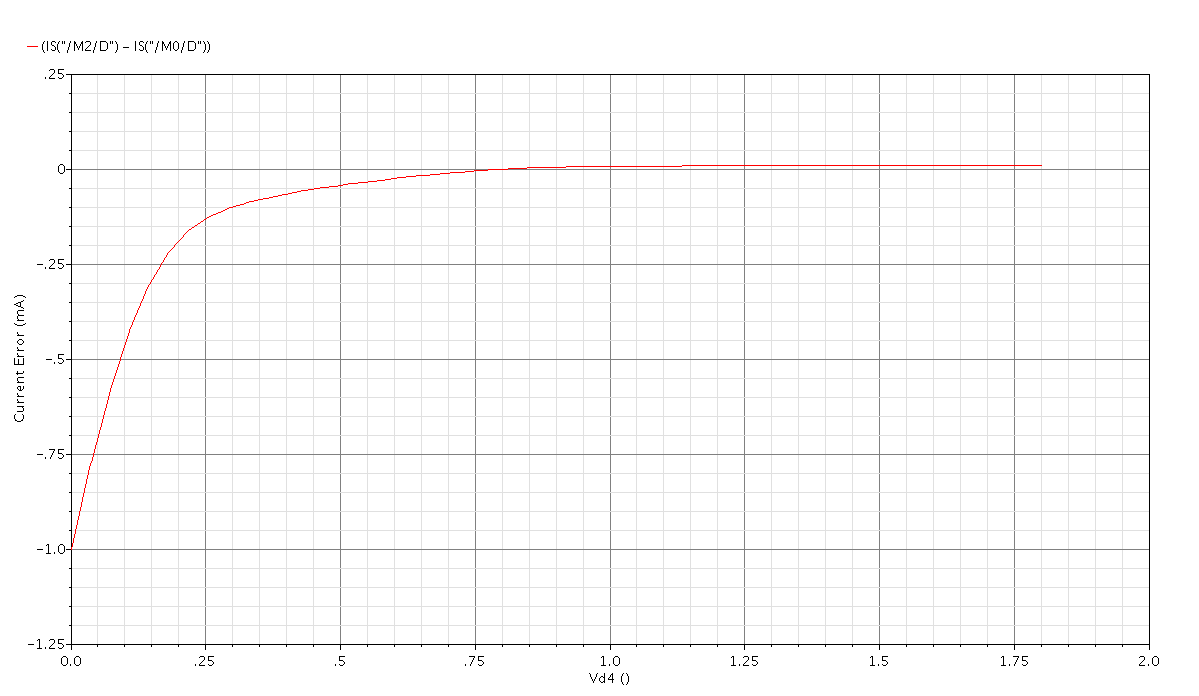
\includegraphics[width=6in]{p2_3_2}
\caption{Current Gain vs. $V_{D-4}$ for the Cascode Current Mirror Configuration}
\label{2_3b}
\end{figure}
\newpage

\subsection{}
\begin{figure}[H]
\centering
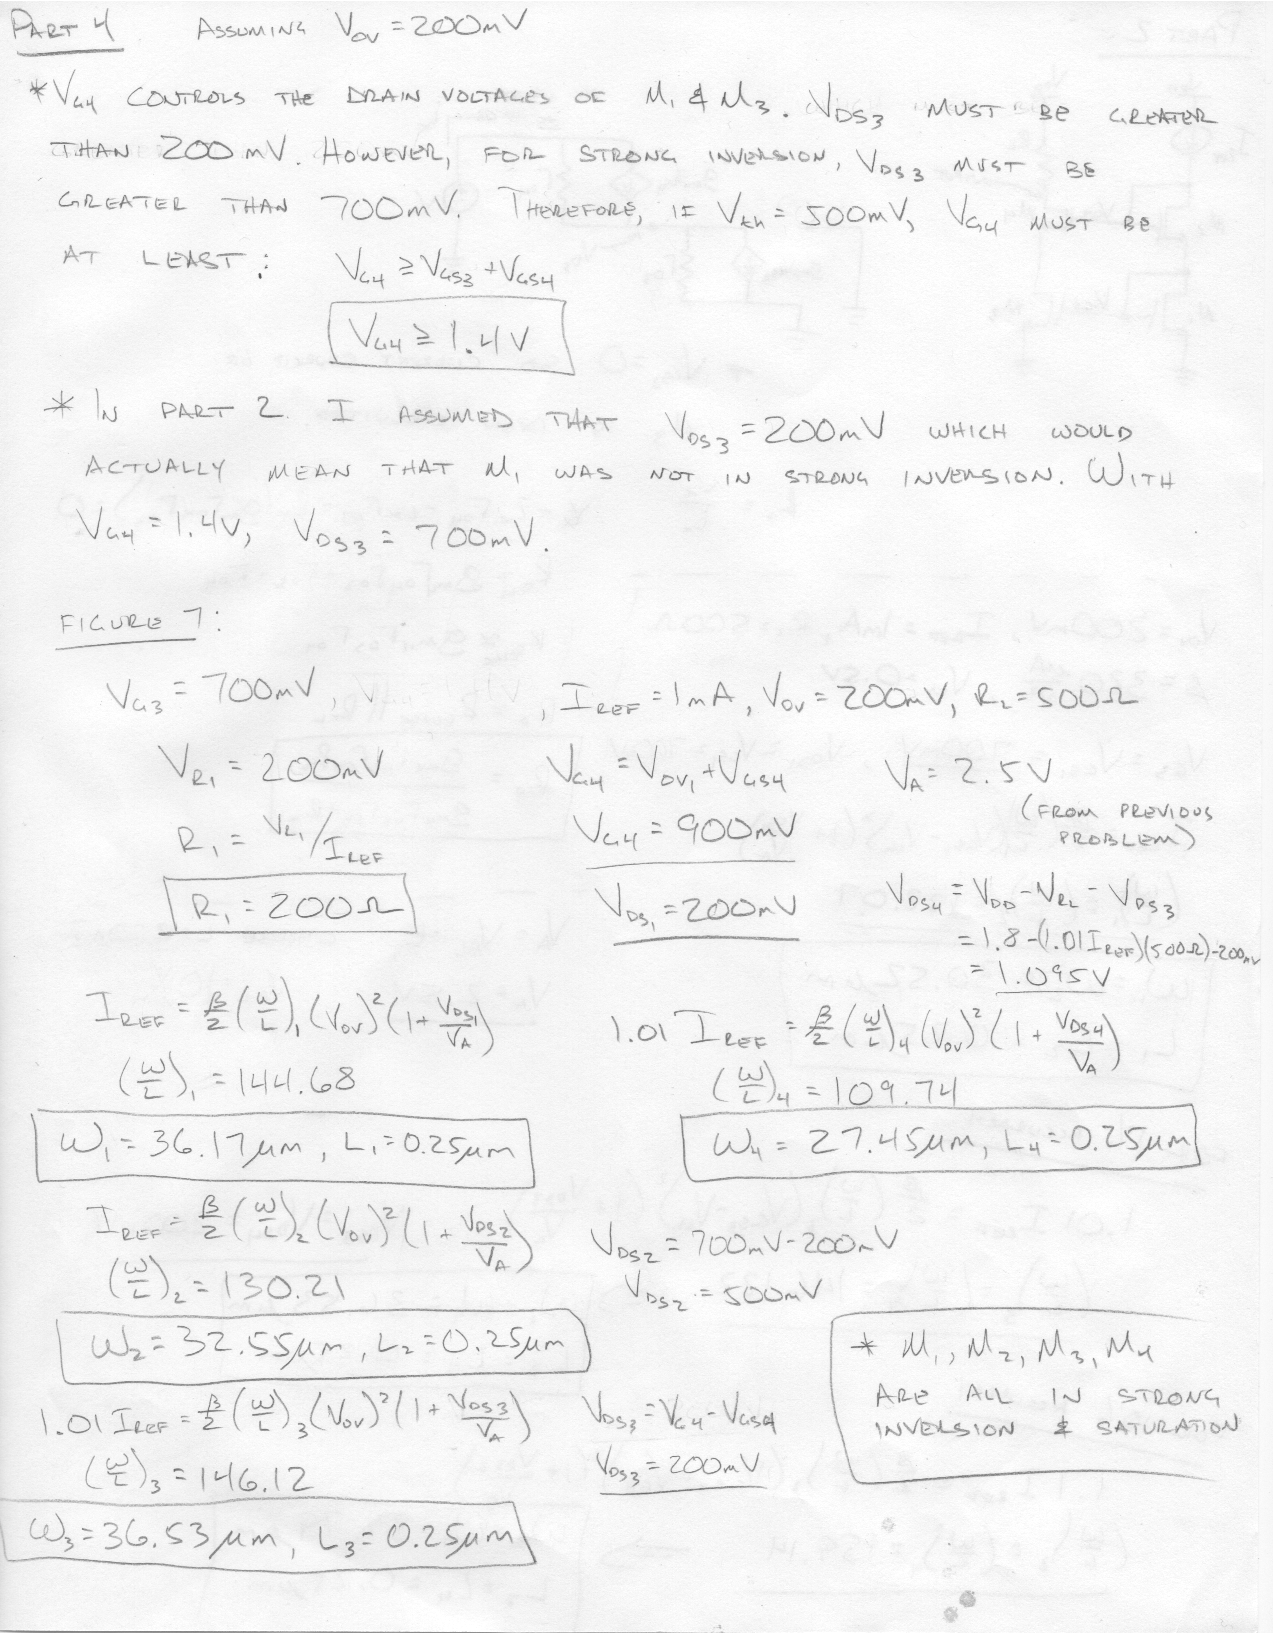
\includegraphics[width=6in]{1_6}
\caption{Hand-Written Work for Problem 2.4}
\label{2_4}
\end{figure}

\begin{figure}[H]
\centering
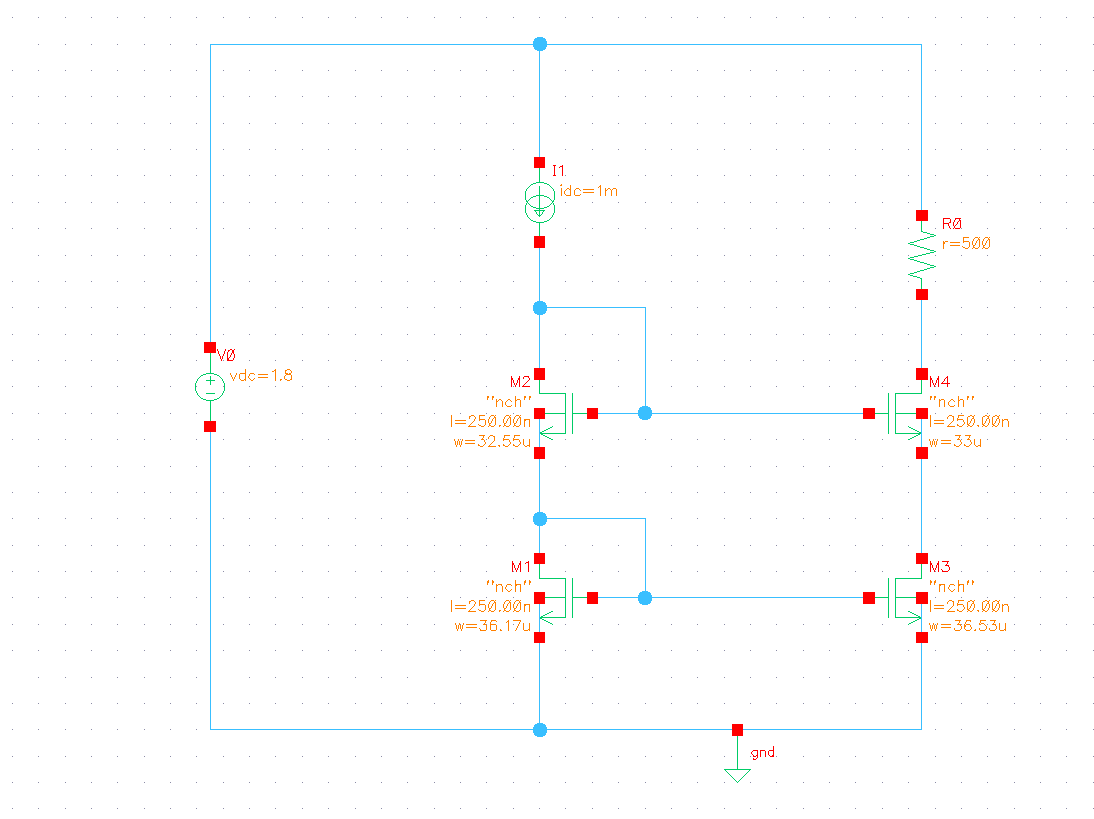
\includegraphics[width=6in]{p2_4_schem.png}
\caption{Schematic to Verify Sizing Calculations}
\label{2_4_schem}
\end{figure}


\begin{figure}[H]
\centering
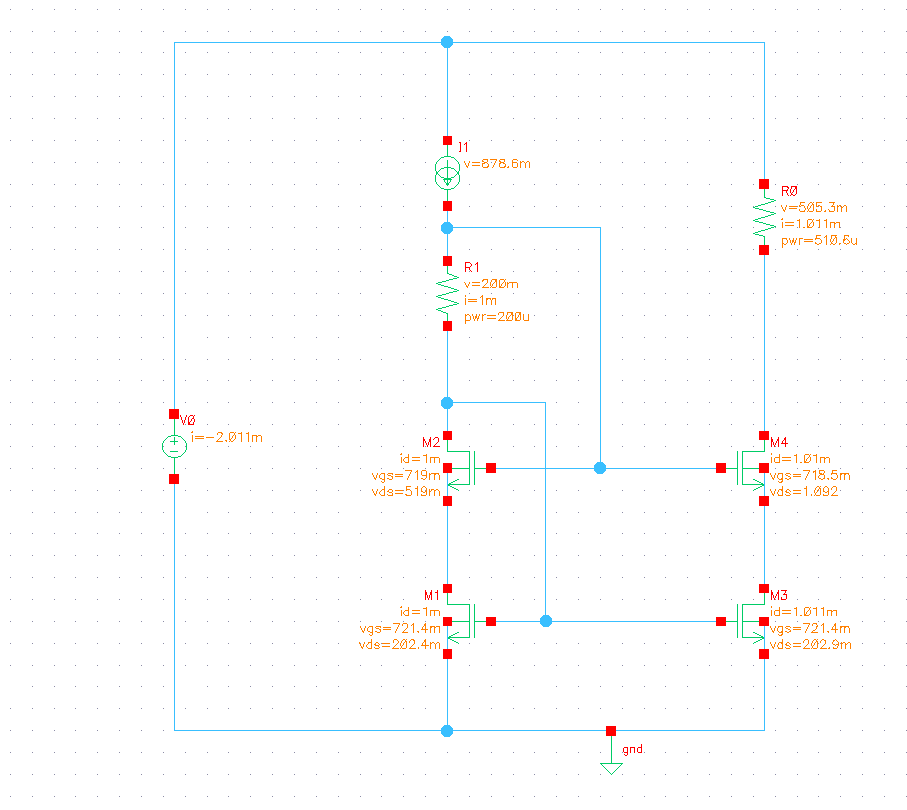
\includegraphics[width=6in]{p2_4_dcop.png}
\caption{Schematic with DC Operating Point Annotations Verifying Sizing Calculations}
\label{2_4_dcop}
\end{figure}
\newpage

\subsection{}
\begin{figure}[H]
\centering
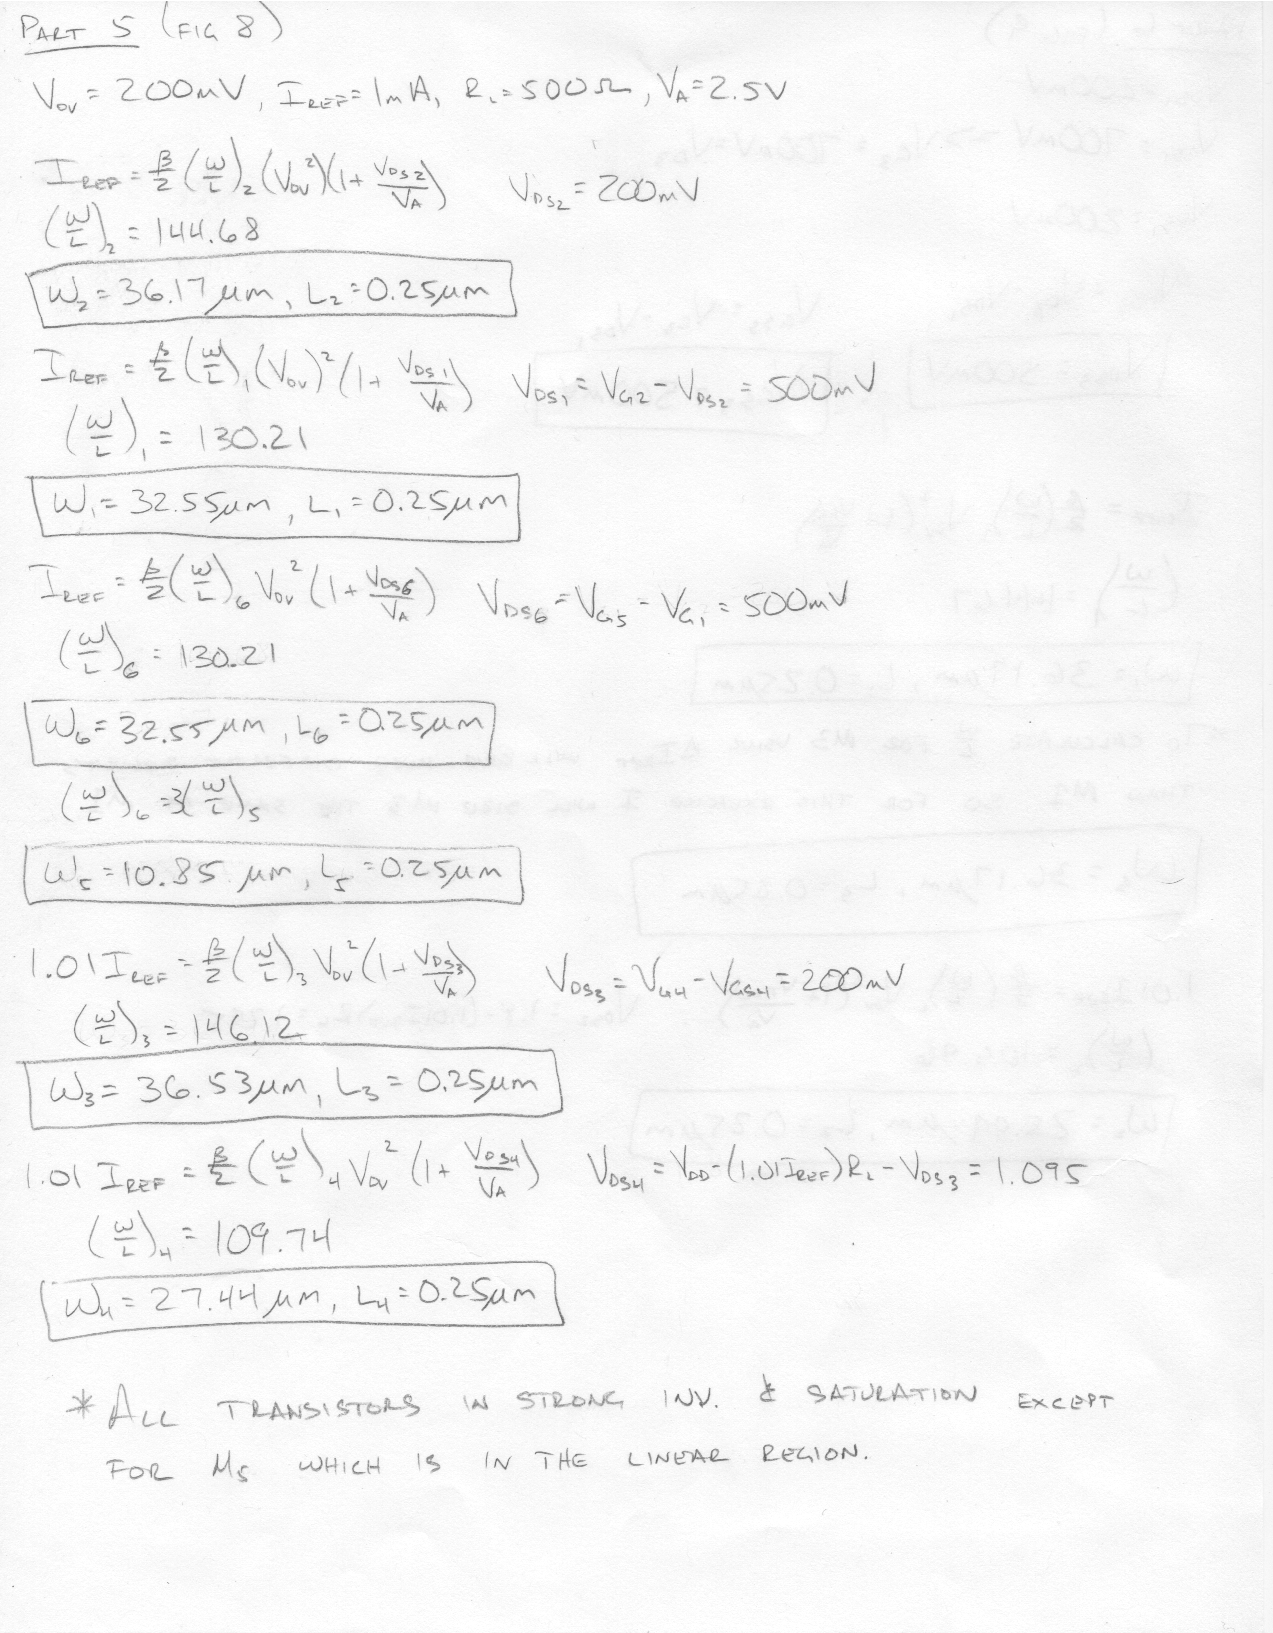
\includegraphics[width=6in]{1_7}
\caption{Hand-Written Work for Problem 2.5}
\label{2_5}
\end{figure}

\begin{figure}[H]
\centering
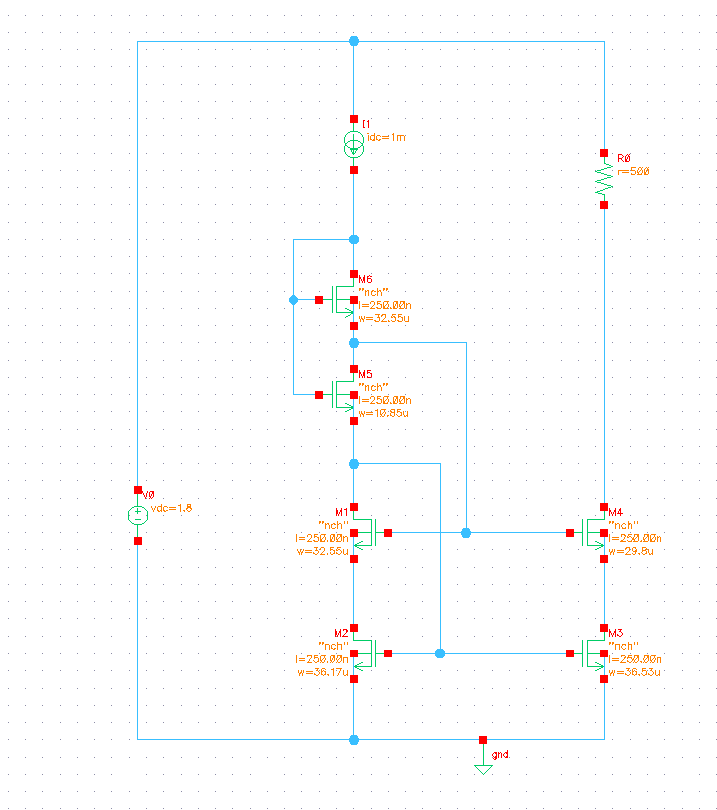
\includegraphics[width=6in]{p2_5_schem.png}
\caption{Schematic to Verify Sizing Calculations}
\label{2_5_schem}
\end{figure}


\begin{figure}[H]
\centering
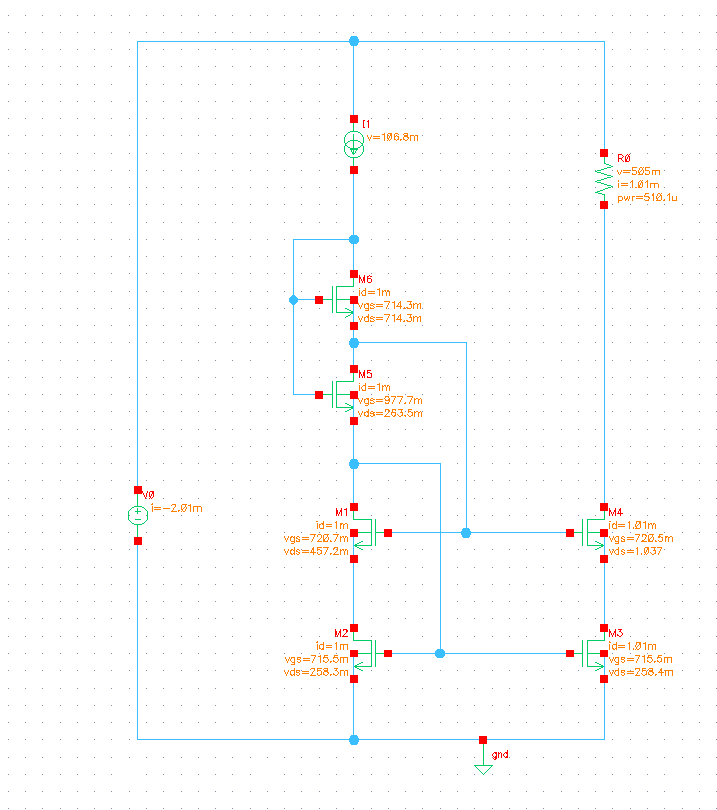
\includegraphics[width=6in]{p2_5_dcop.png}
\caption{Schematic with DC Operating Point Annotations Verifying Sizing Calculations}
\label{2_5_dcop}
\end{figure}
\newpage

\subsection{}
\begin{figure}[H]
\centering
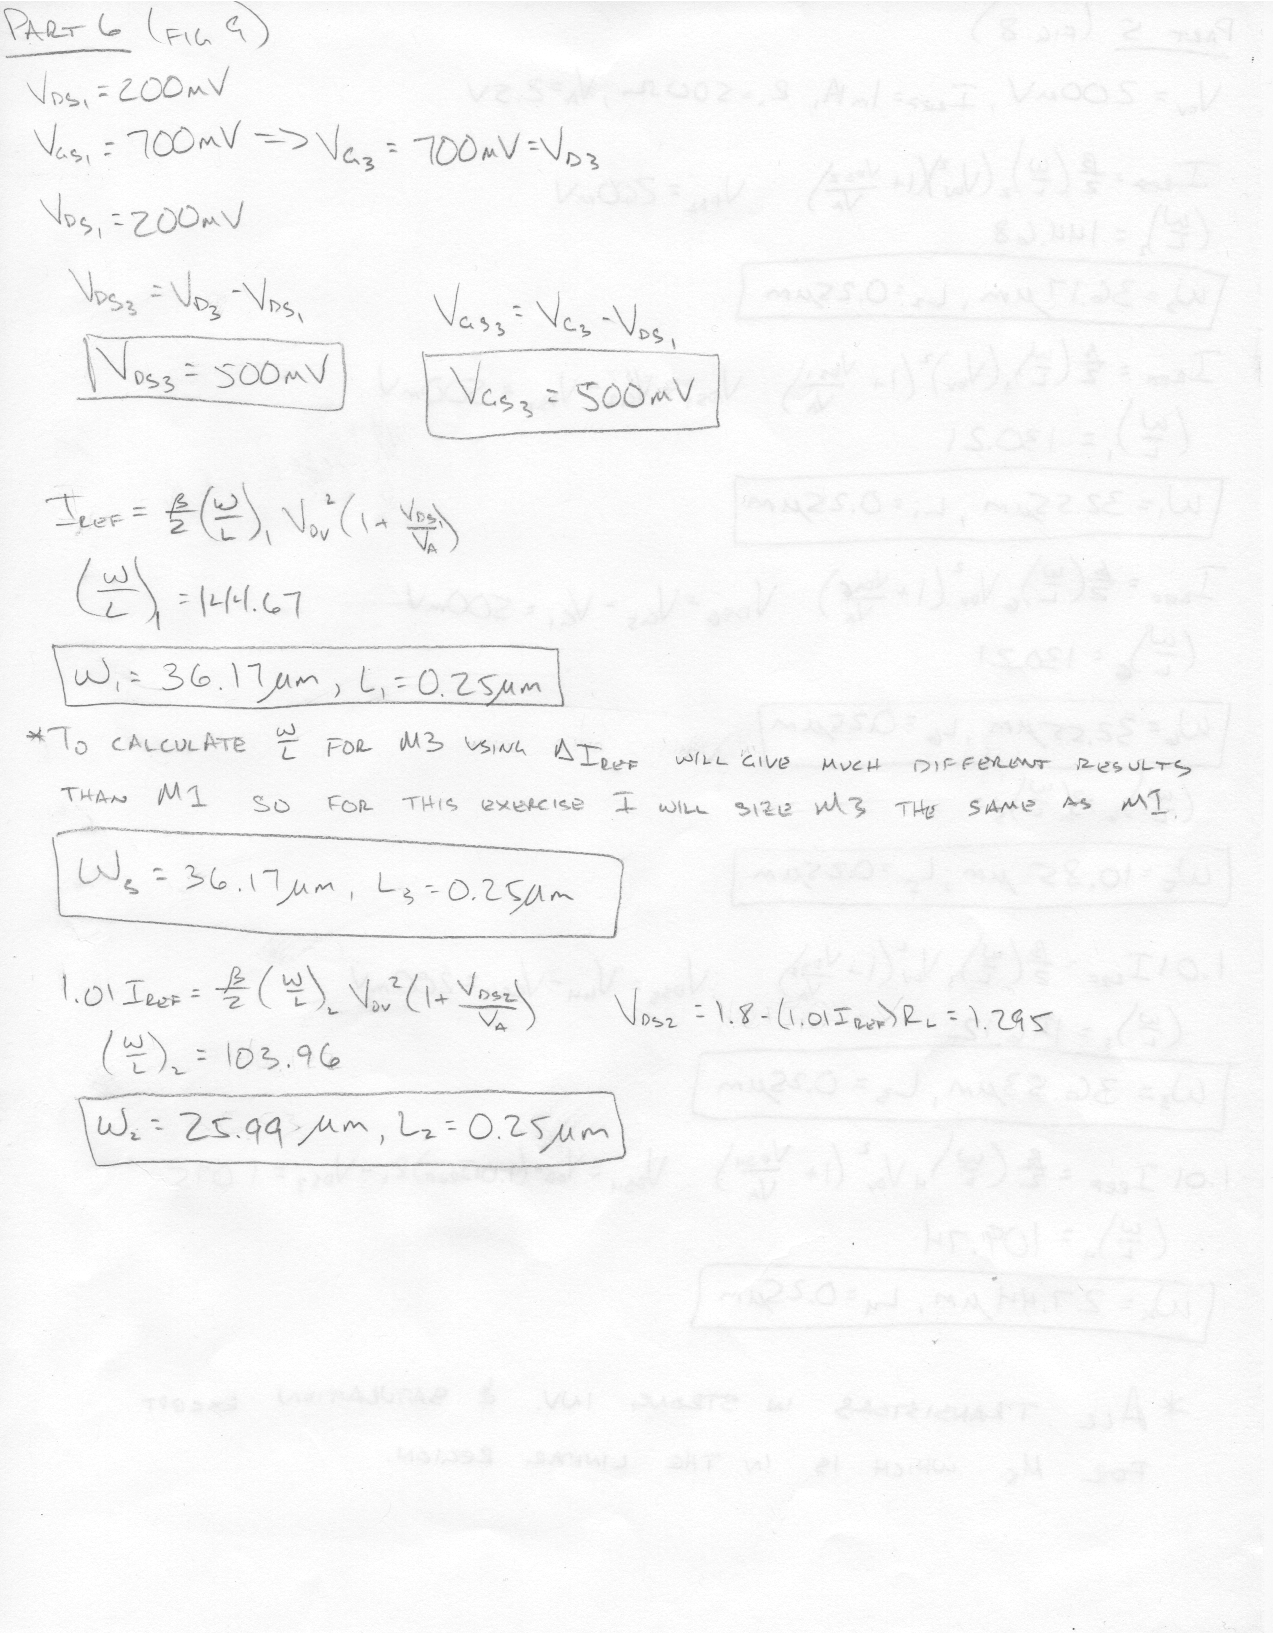
\includegraphics[width=6in]{1_8}
\caption{Hand-Written Work for Problem 2.6}
\label{2_6}
\end{figure}

\begin{figure}[H]
\centering
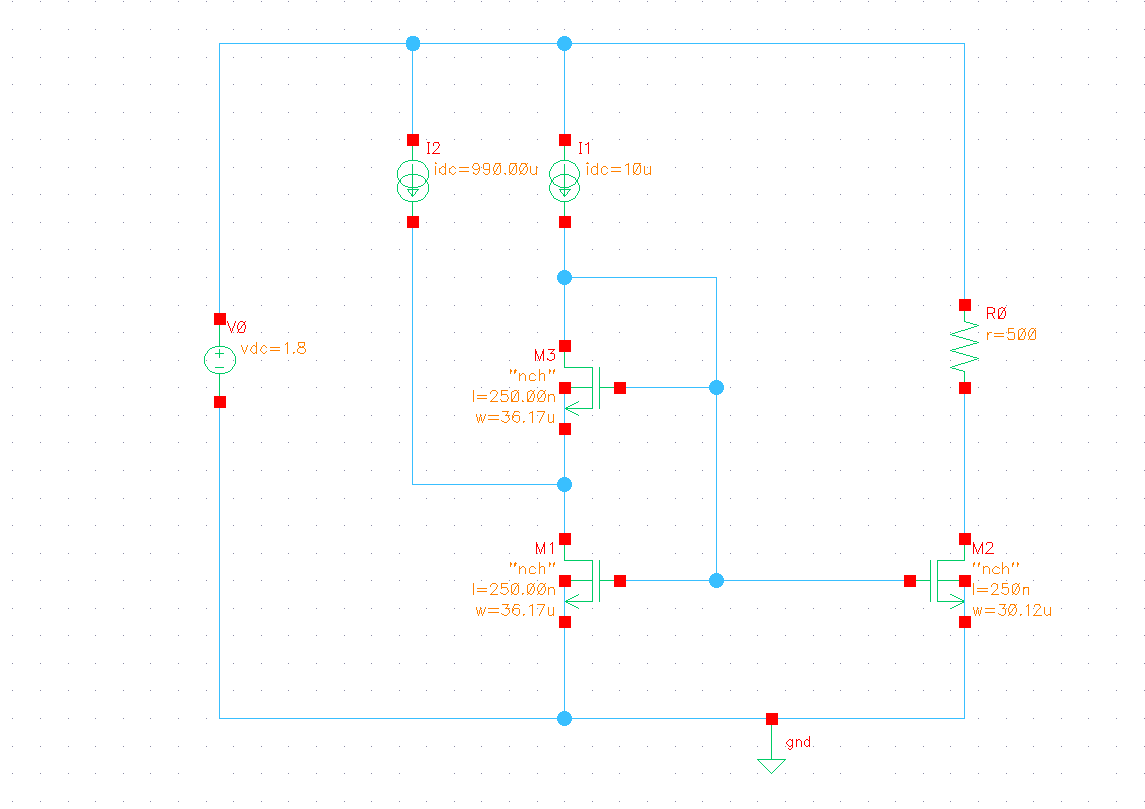
\includegraphics[width=6in]{p2_6_schem.png}
\caption{Schematic to Verify Sizing Calculations}
\label{2_6_schem}
\end{figure}


\begin{figure}[H]
\centering
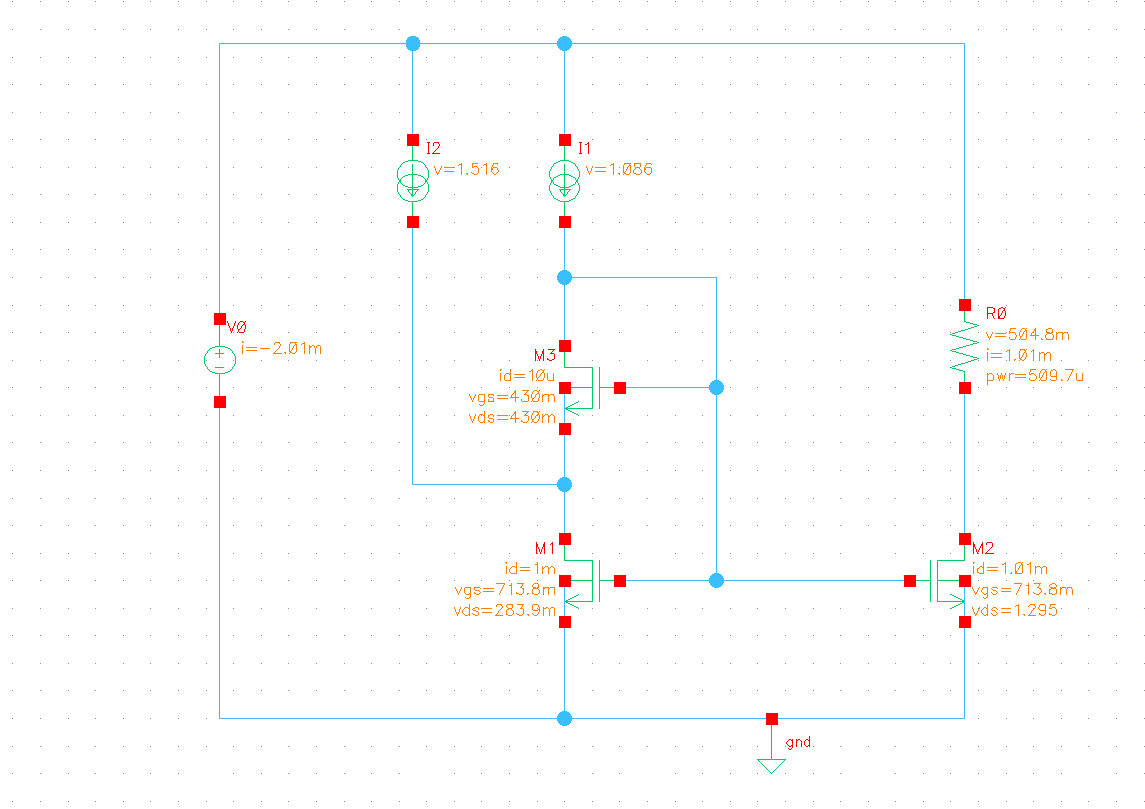
\includegraphics[width=6in]{p2_6_dcop.png}
\caption{Schematic with DC Operating Point Annotations Verifying Sizing Calculations}
\label{2_6_dcop}
\end{figure}
\newpage

\section{Problem 3}
\subsection{}

\begin{figure}[H]
\centering
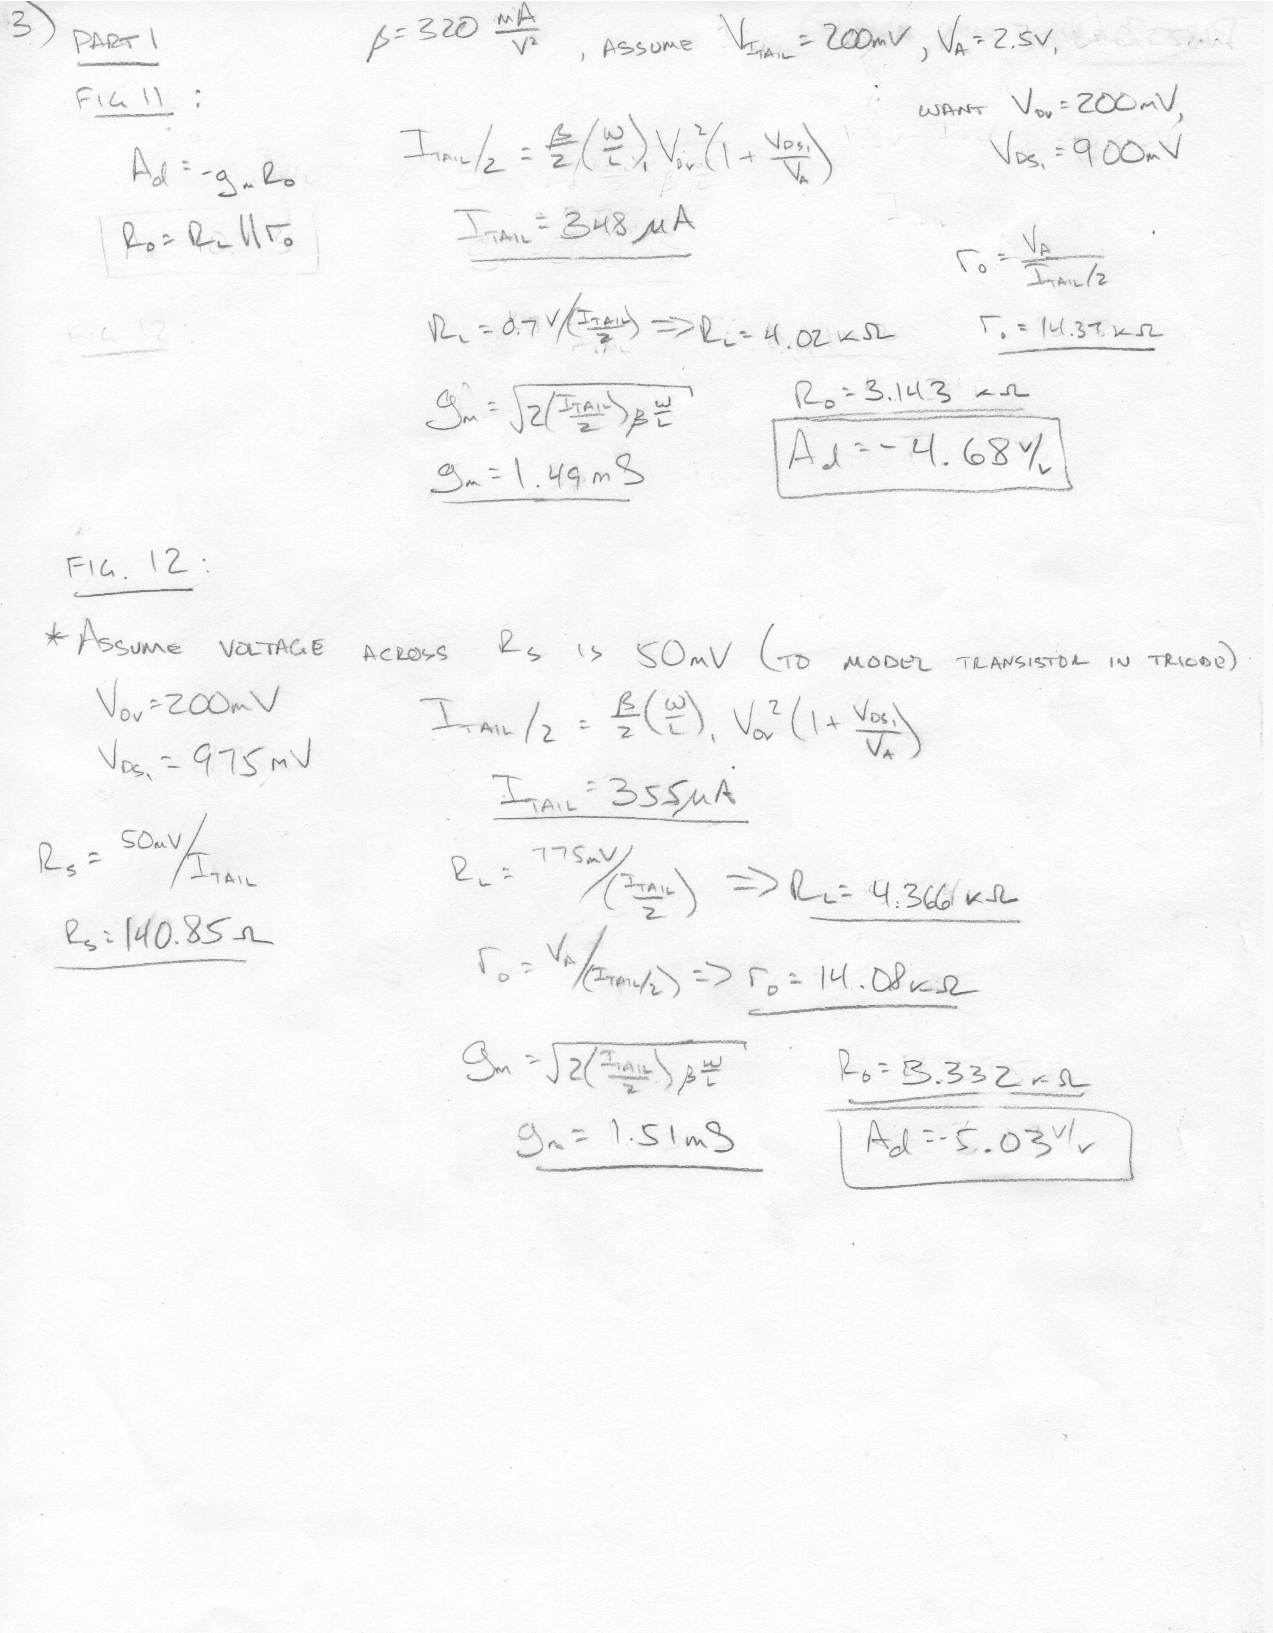
\includegraphics[width=6in]{1_9}
\caption{Hand-Written Work for Problem 3.1}
\label{3_1}
\end{figure}

\begin{figure}[H]
\centering
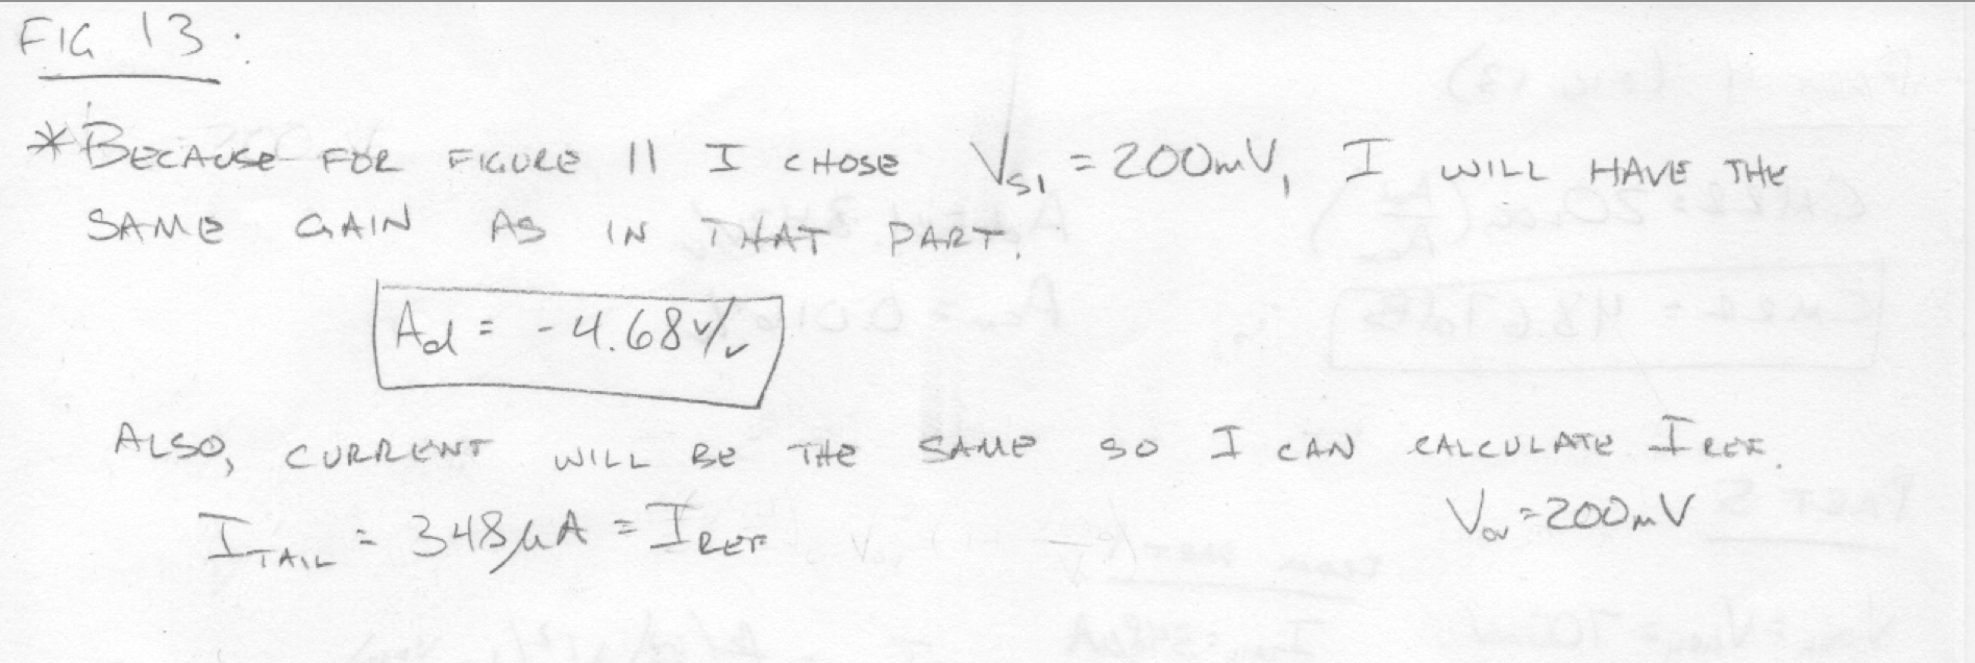
\includegraphics[width=6in]{1_9a}
\caption{Hand-Written Work for Problem 3.1 (cntd)}
\label{3_1a}
\end{figure}

\begin{figure}[H]
\centering
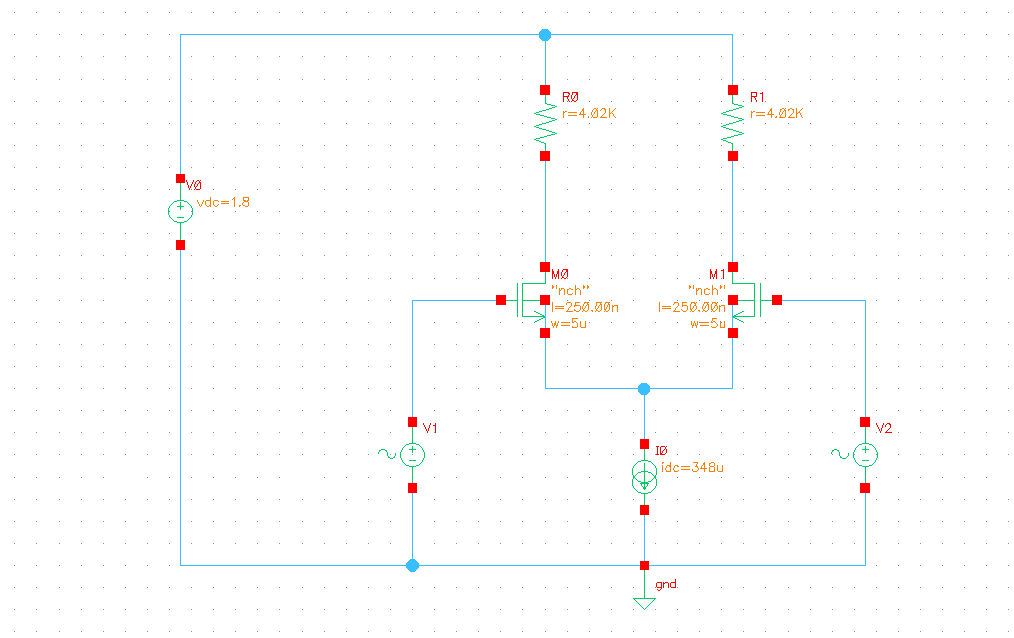
\includegraphics[width=6in]{p3_1a_schem}
\caption{Schematic to Verifying Gain Calculations for Figure 11}
\label{3_1a_schem}
\end{figure}

\begin{figure}[H]
\centering
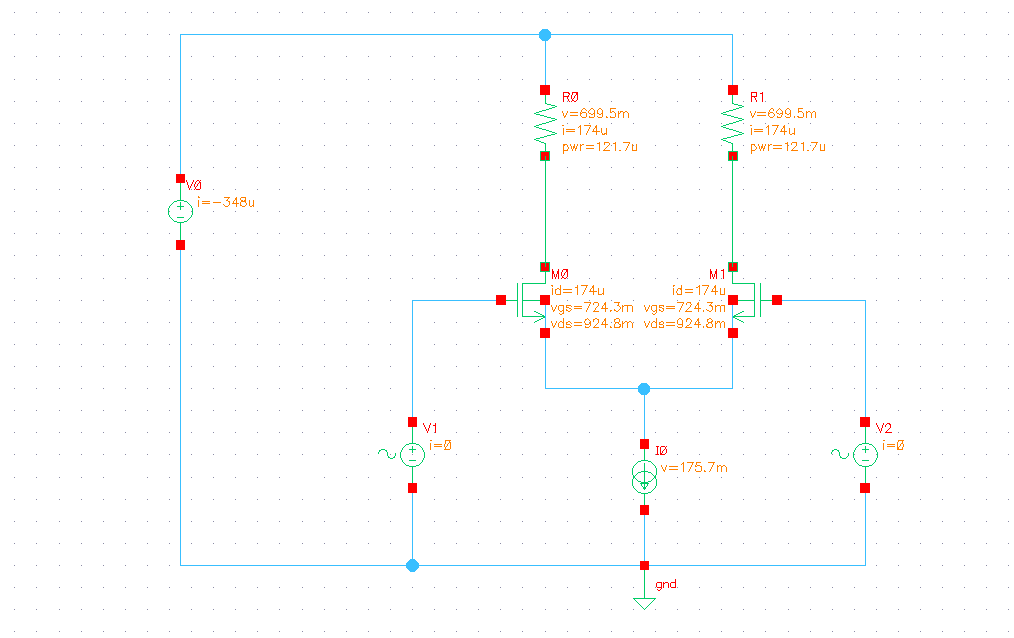
\includegraphics[width=6in]{p3_1a_dcop}
\caption{Schematic with DC Operating Point Annotations to Verifying Gain Calculations for Figure 11}
\label{3_1a_dcop}
\end{figure}

\begin{figure}[H]
\centering
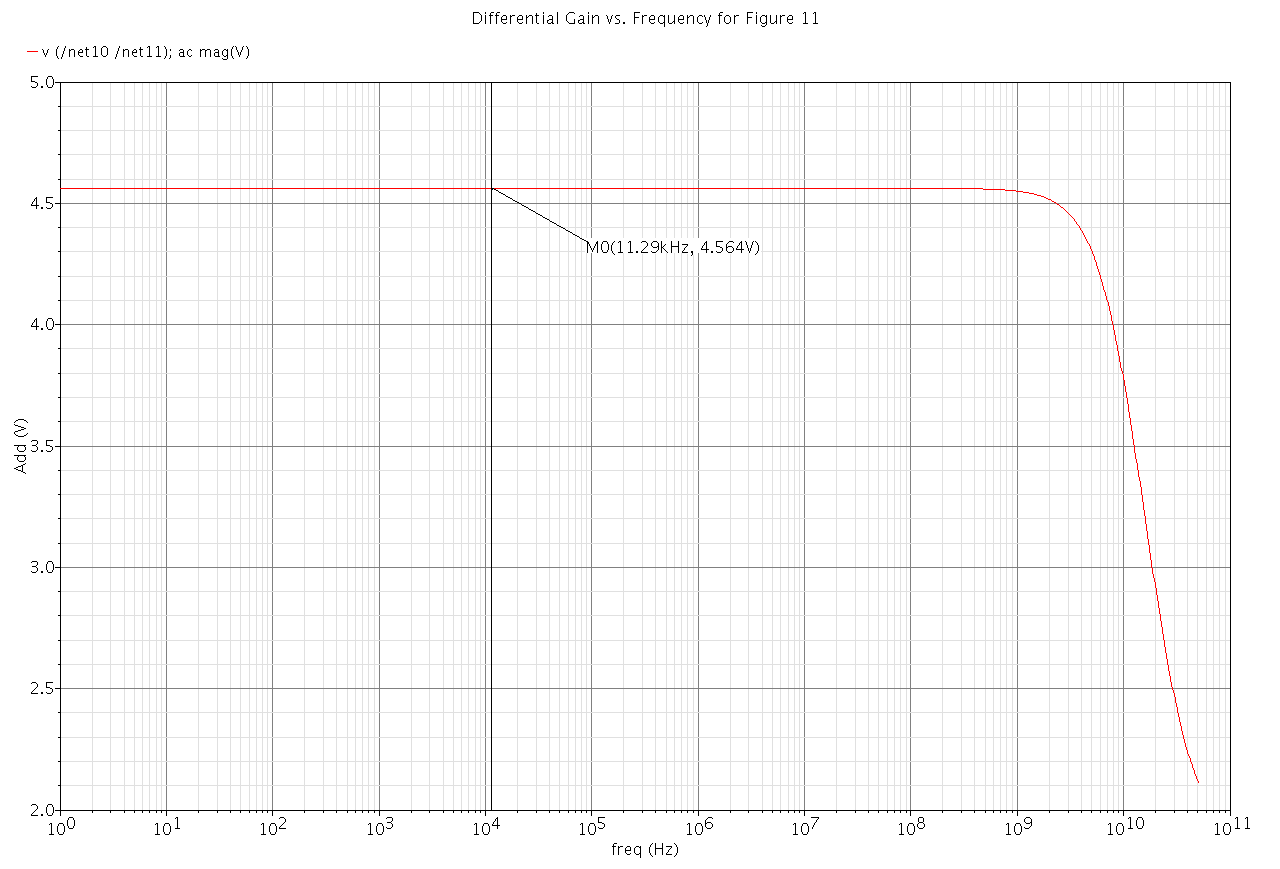
\includegraphics[width=6in]{p3_1a_gain}
\caption{Gain vs. Frequency for Figure 11}
\label{3_1a_gain}
\end{figure}

\begin{figure}[H]
\centering
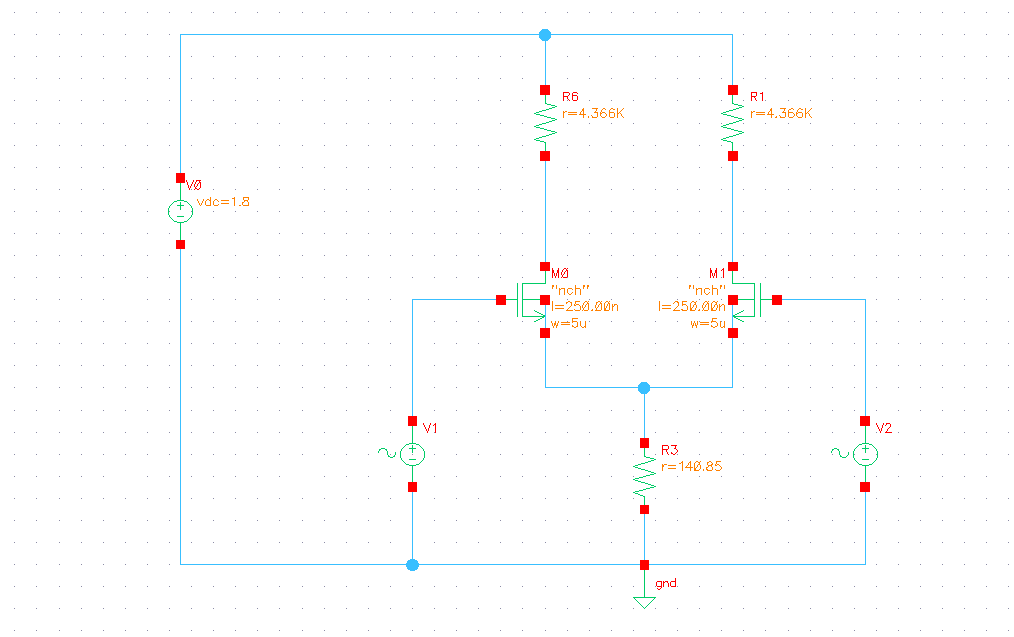
\includegraphics[width=6in]{p3_1b_schem}
\caption{Schematic to Verifying Gain Calculations for Figure 12}
\label{3_1b_schem}
\end{figure}

\begin{figure}[H]
\centering
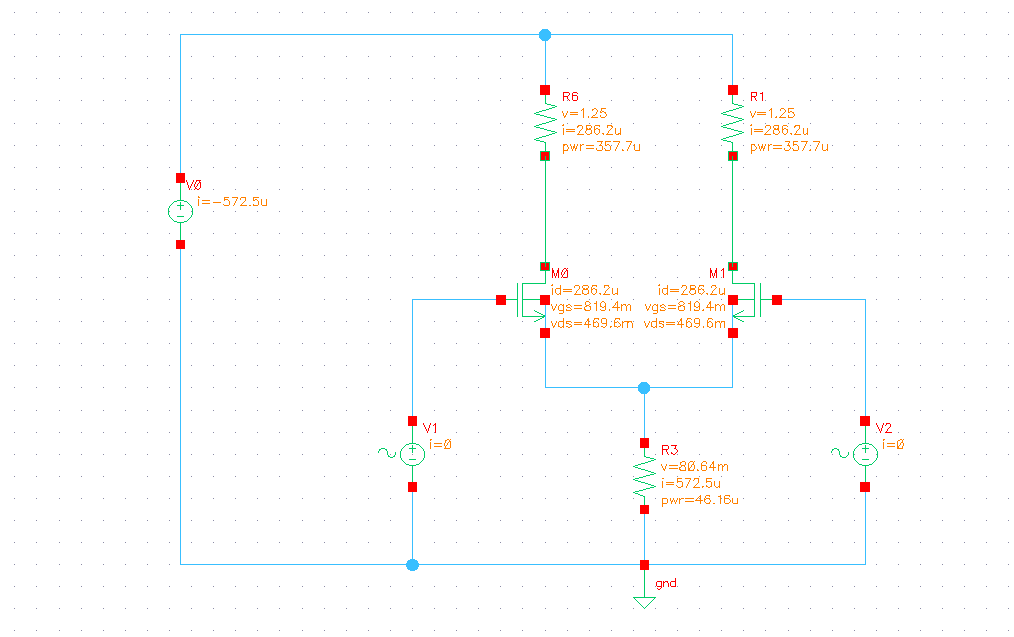
\includegraphics[width=6in]{p3_1b_dcop}
\caption{Schematic with DC Operating Point Annotations to Verifying Gain Calculations for Figure 12}
\label{3_1b_dcop}
\end{figure}

\begin{figure}[H]
\centering
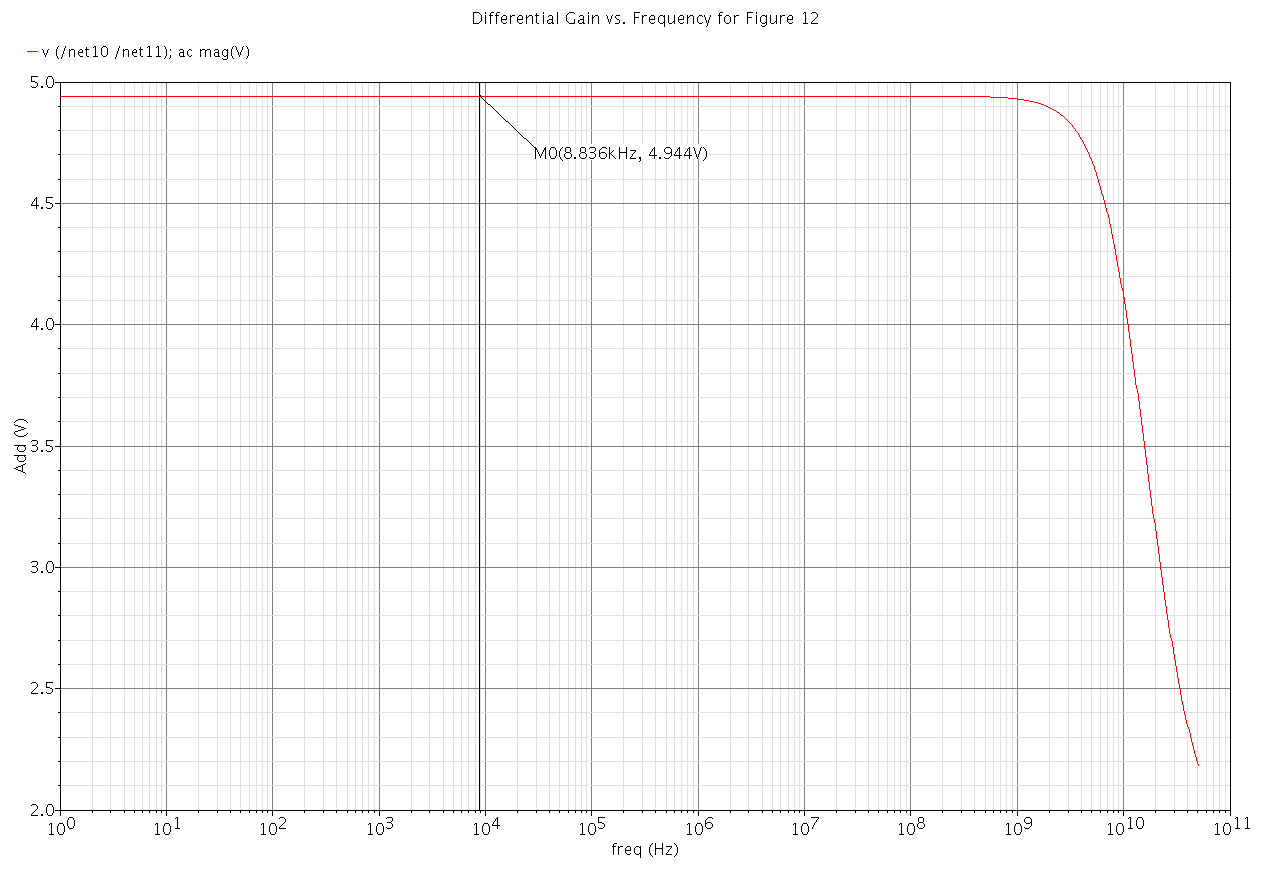
\includegraphics[width=6in]{p3_1b_gain}
\caption{Gain vs. Frequency for Figure 12}
\label{3_1b_gain}
\end{figure}

\begin{figure}[H]
\centering
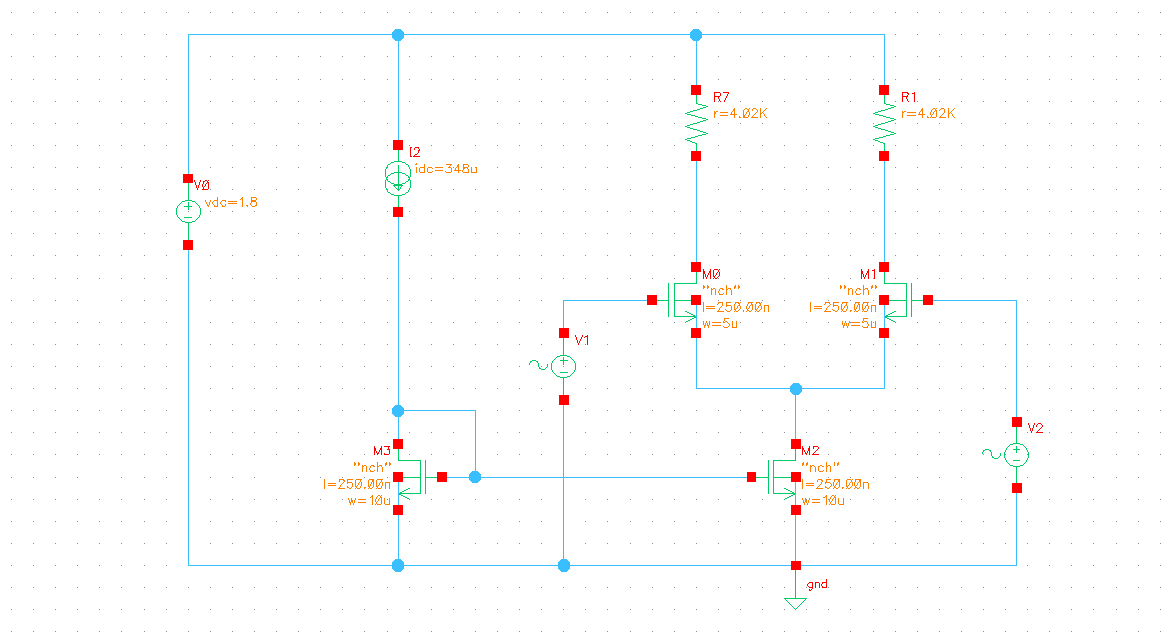
\includegraphics[width=6in]{p3_1c_schem}
\caption{Schematic to Verifying Gain Calculations for Figure 13}
\label{3_1c_schem}
\end{figure}

\begin{figure}[H]
\centering
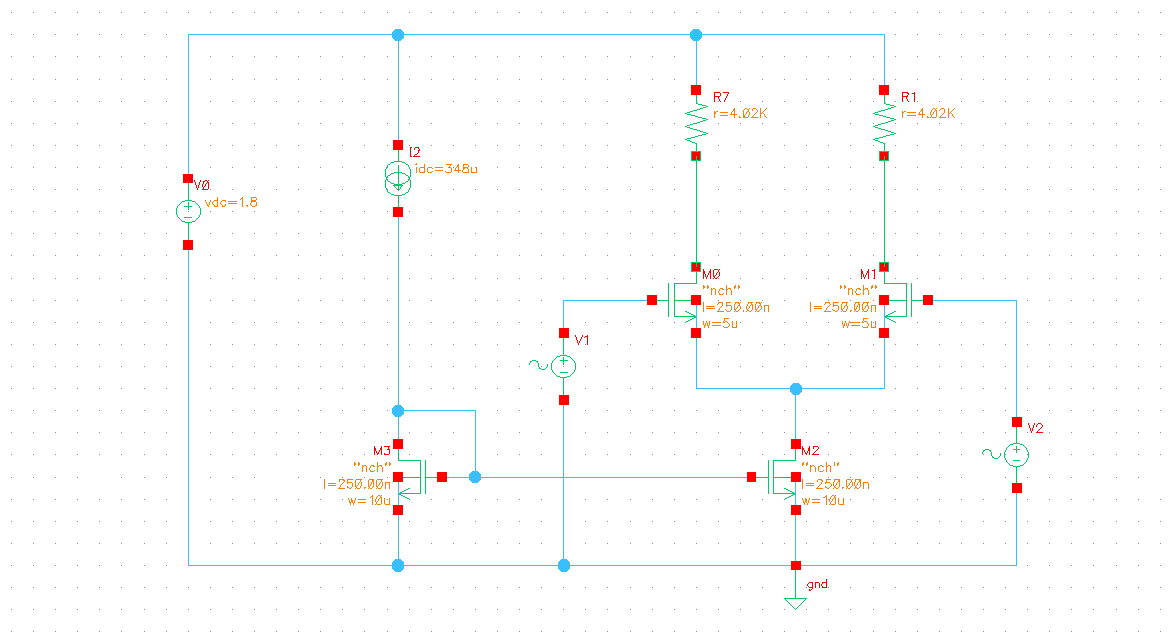
\includegraphics[width=6in]{p3_1c_dcop}
\caption{Schematic with DC Operating Point Annotations to Verifying Gain Calculations for Figure 13}
\label{3_1c_dcop}
\end{figure}

\begin{figure}[H]
\centering
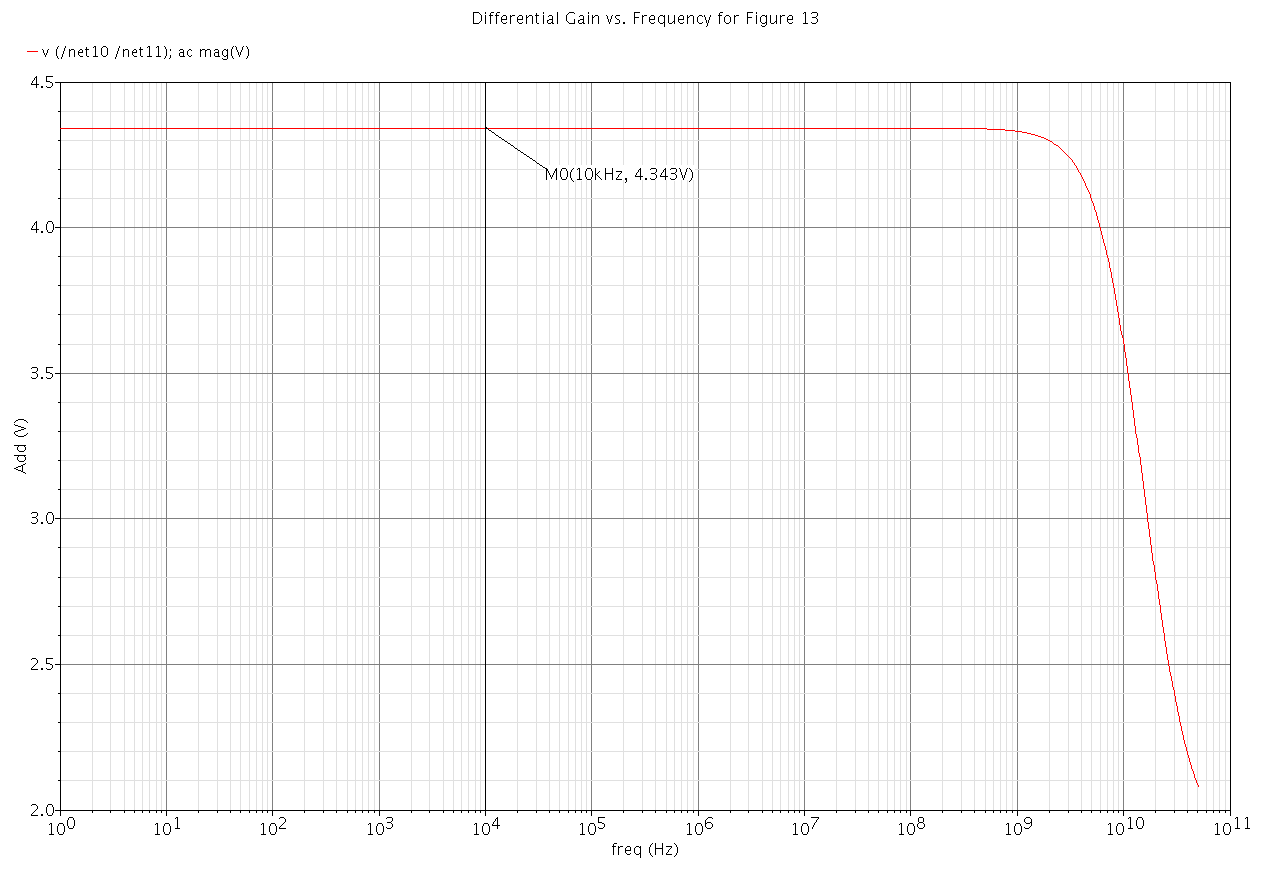
\includegraphics[width=6in]{p3_1c_gain}
\caption{Gain vs. Frequency for Figure 13}
\label{3_1c_gain}
\end{figure}
\newpage

\subsection{}
In this problem I plotted the I-V transfer characteristics for the three differential stages. The first utilizes an ideal current source and thus has a close to perfect butterfly diagram plot. The second utilizes a resistor current source which does not hold the total current through the pair steady. As can be seen, the current actually rises above the $20\mu A$ current initially calculated. However, the butterfly curve can still be seen in the transfer characteristic of this configuration. The third circuit utilizes a current mirror source. Because the transistor cannot act as a perfect current source, the current never saturates and continues to rise as the dean voltage of M0 rises (as a result of the gate voltage of the "ON" transistor at any given time). Also, there is a section of the plot where both currents are off which is a result of the ~500mV threshold voltage of each device.

The required voltage to switch on just one of the the input transistors as discussed in class is
\begin{equation}
V_{ON} = \sqrt{2}V_{OV} = 0.28V
\end{equation}.

\begin{figure}[H]
\centering
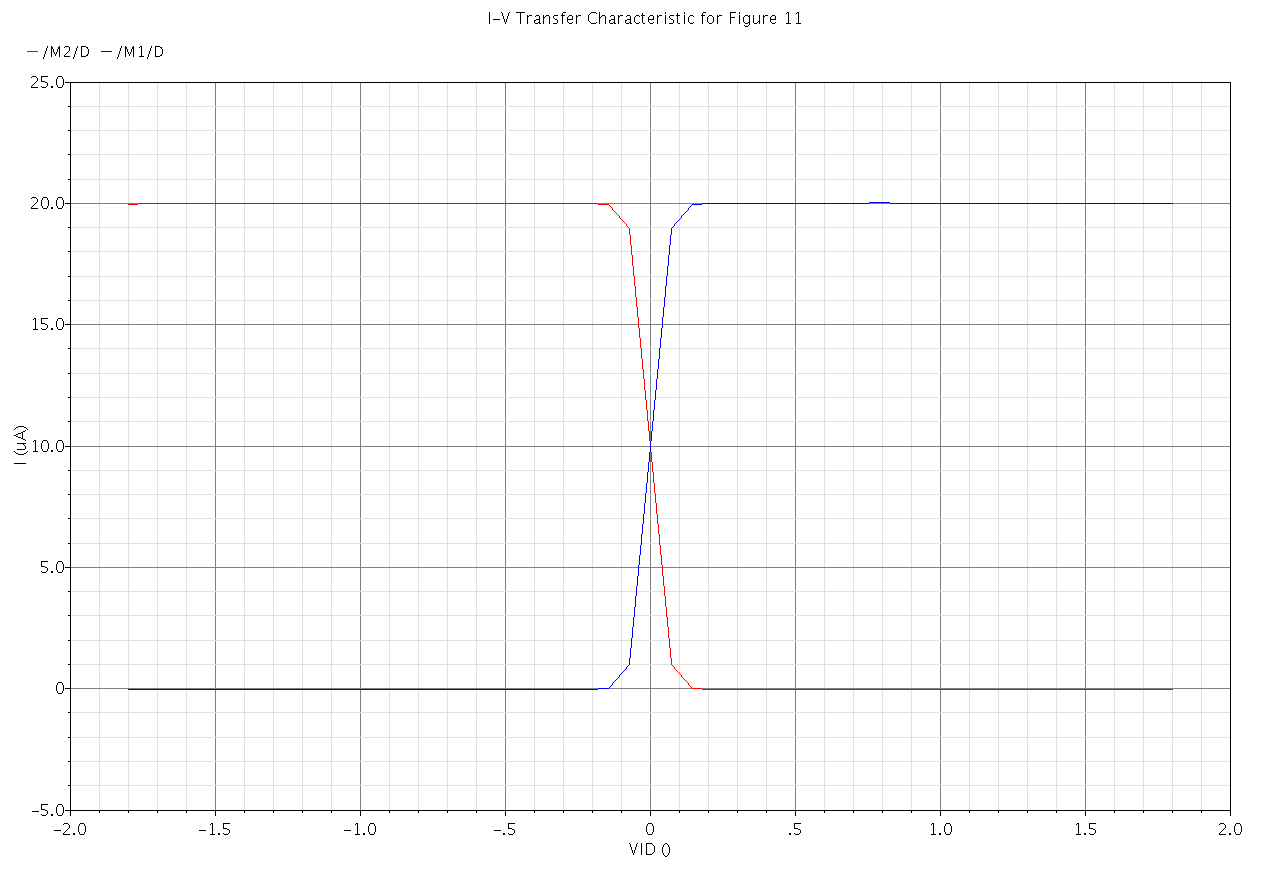
\includegraphics[width=6in]{p3_2a}
\caption{Current Through Each Transistor of the Diff Pair in Figure 11 vs. Differential Input Voltage}
\label{3_2a}
\end{figure}

\begin{figure}[H]
\centering
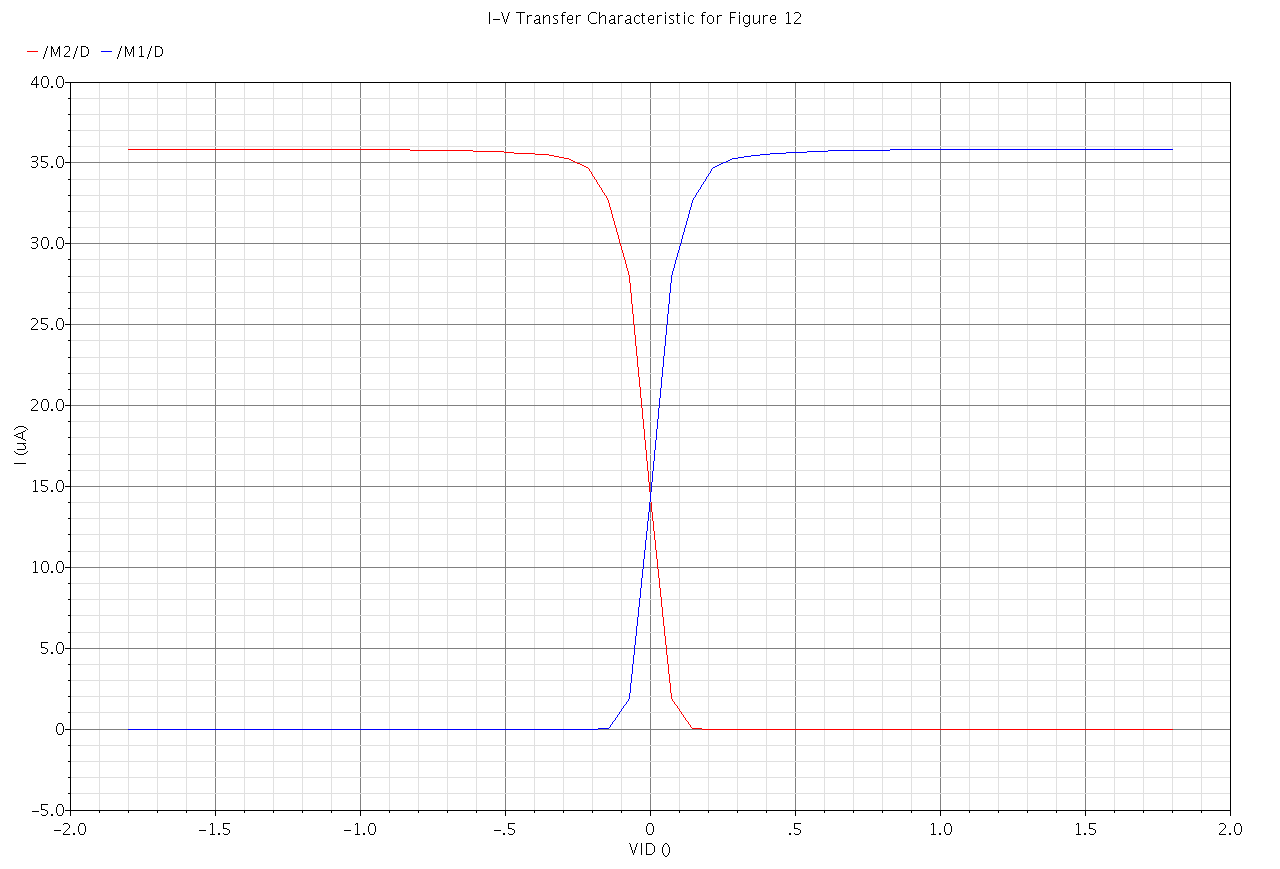
\includegraphics[width=6in]{p3_2b}
\caption{Current Through Each Transistor of the Diff Pair in Figure 12 vs. Differential Input Voltage}
\label{3_2b}
\end{figure}

\begin{figure}[H]
\centering
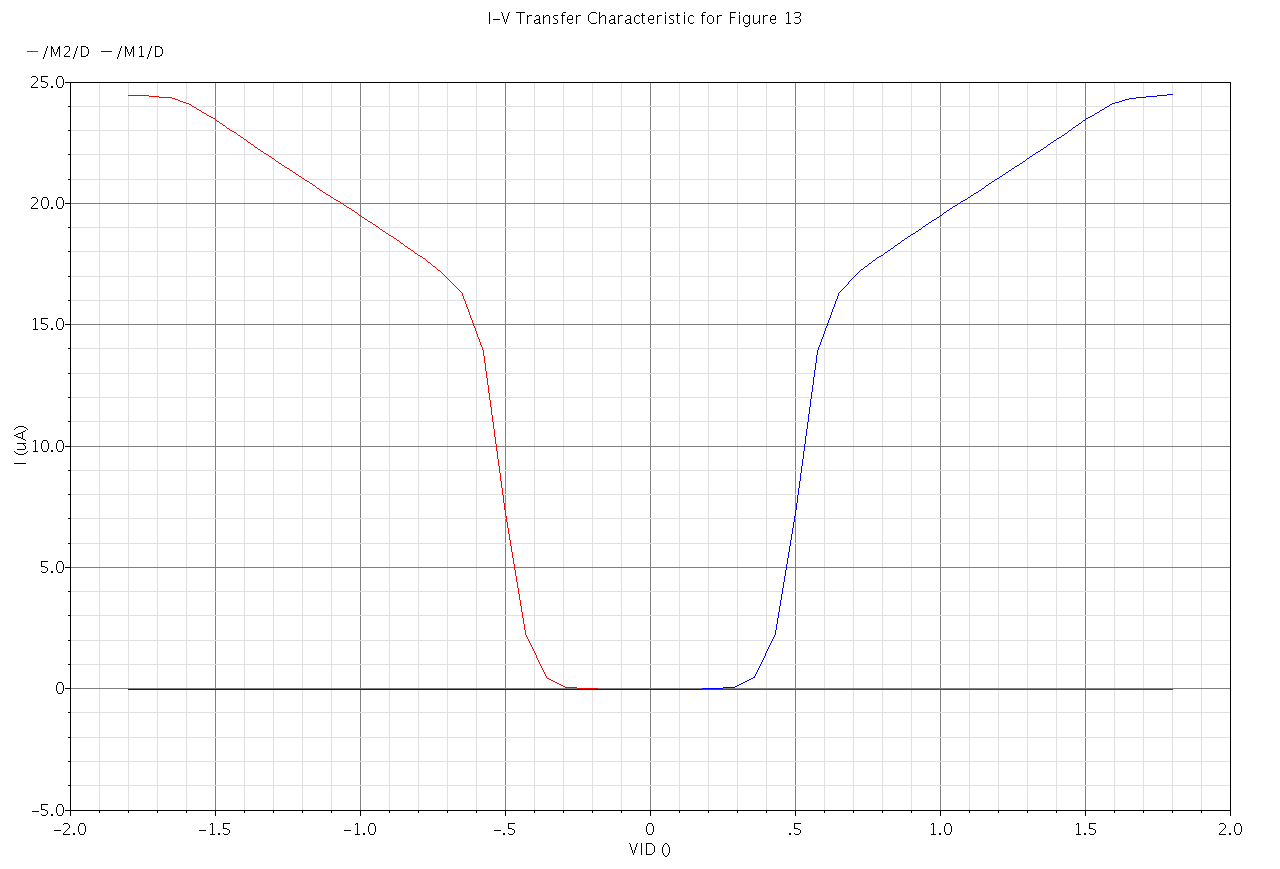
\includegraphics[width=6in]{p3_2c}
\caption{Current Through Each Transistor of the Diff Pair in Figure 13 vs. Differential Input Voltage}
\label{3_2c}
\end{figure}

\subsection{}

\begin{figure}[H]
\centering
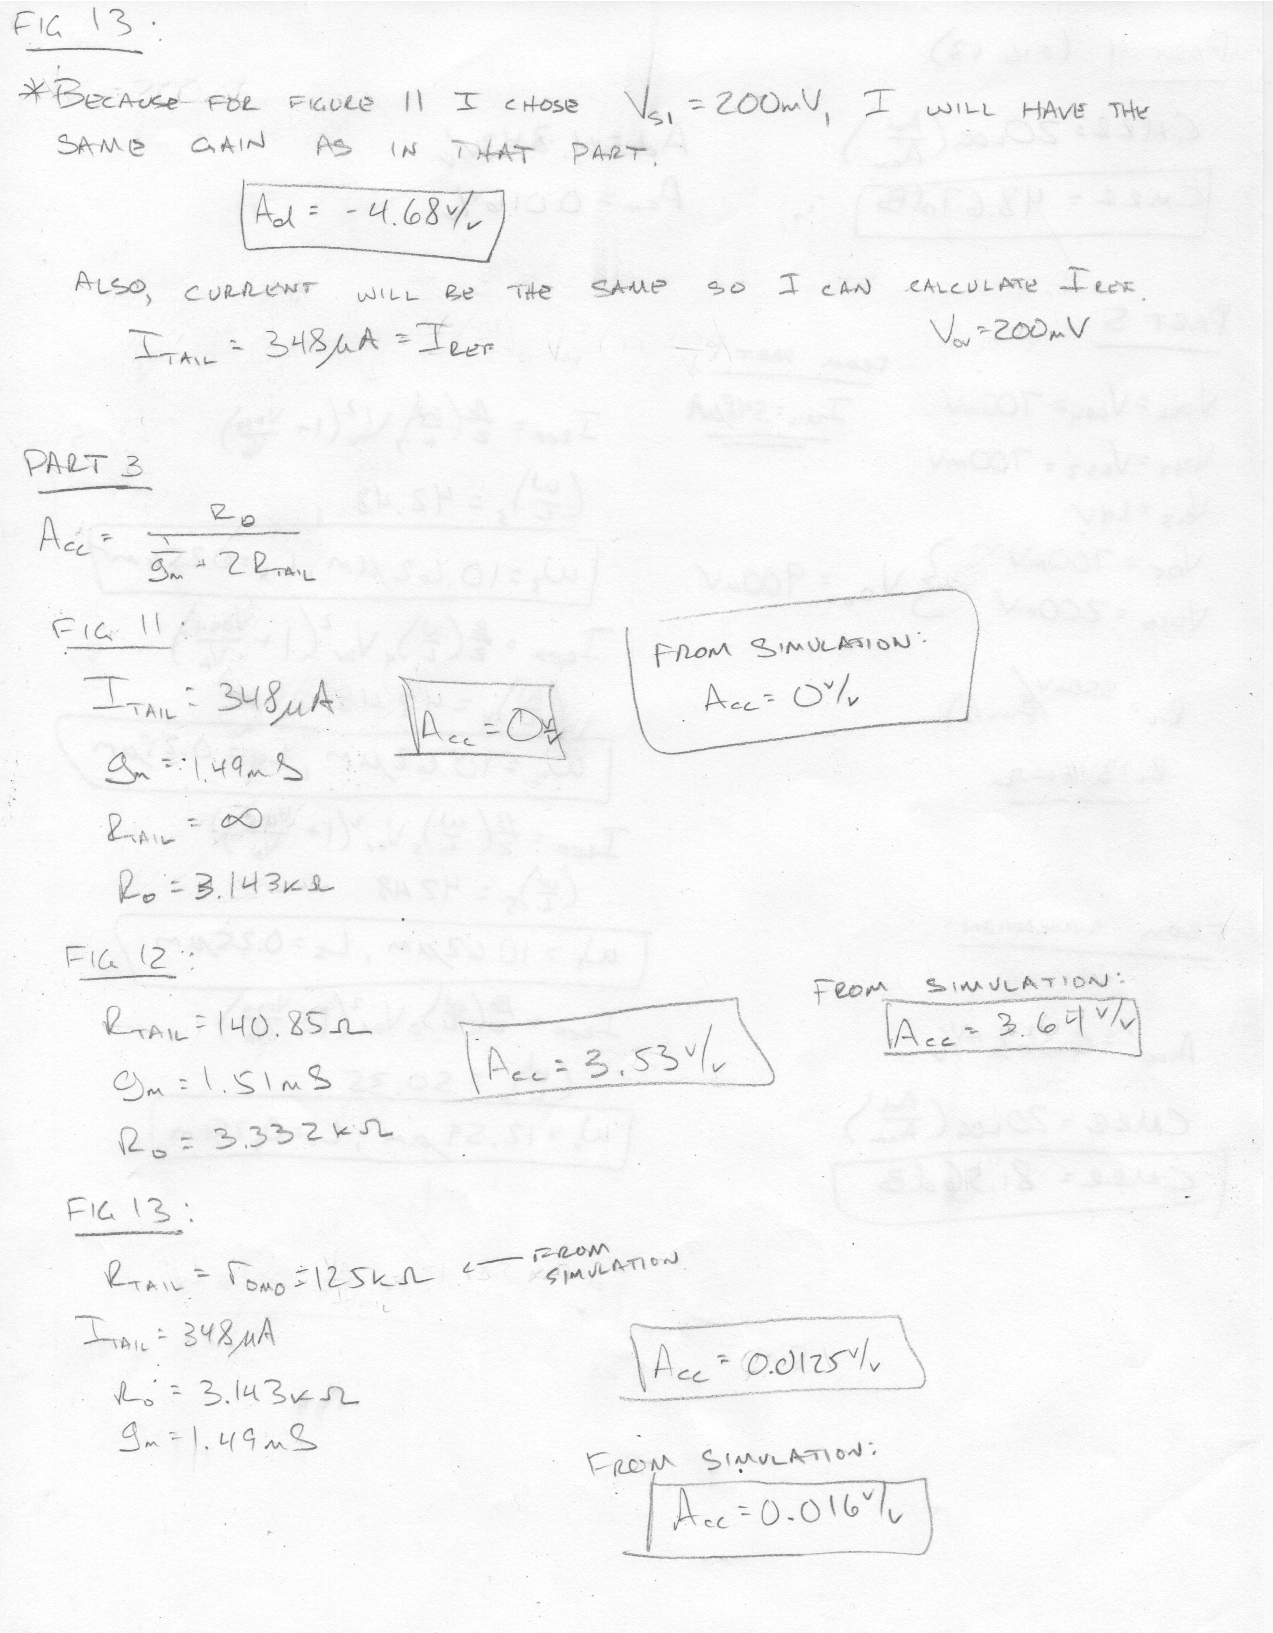
\includegraphics[width=6in]{1_10}
\caption{Hand-Written Work for Problem 3.3}
\label{3_3}
\end{figure}

\begin{figure}[H]
\centering
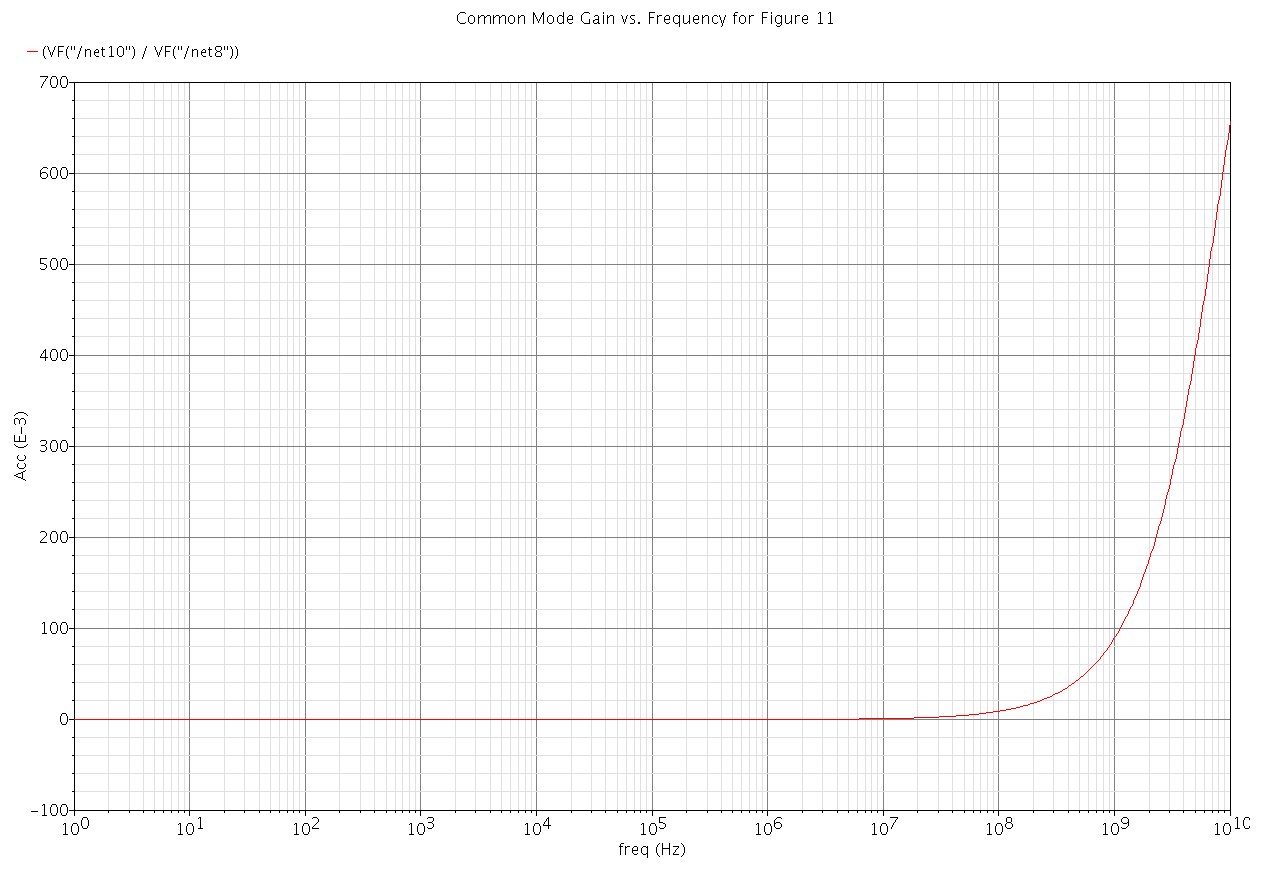
\includegraphics[width=6in]{p3_3a}
\caption{Common Mode Gain vs. Frequency for Figure 11}
\label{3_3a_gain}
\end{figure}

\begin{figure}[H]
\centering
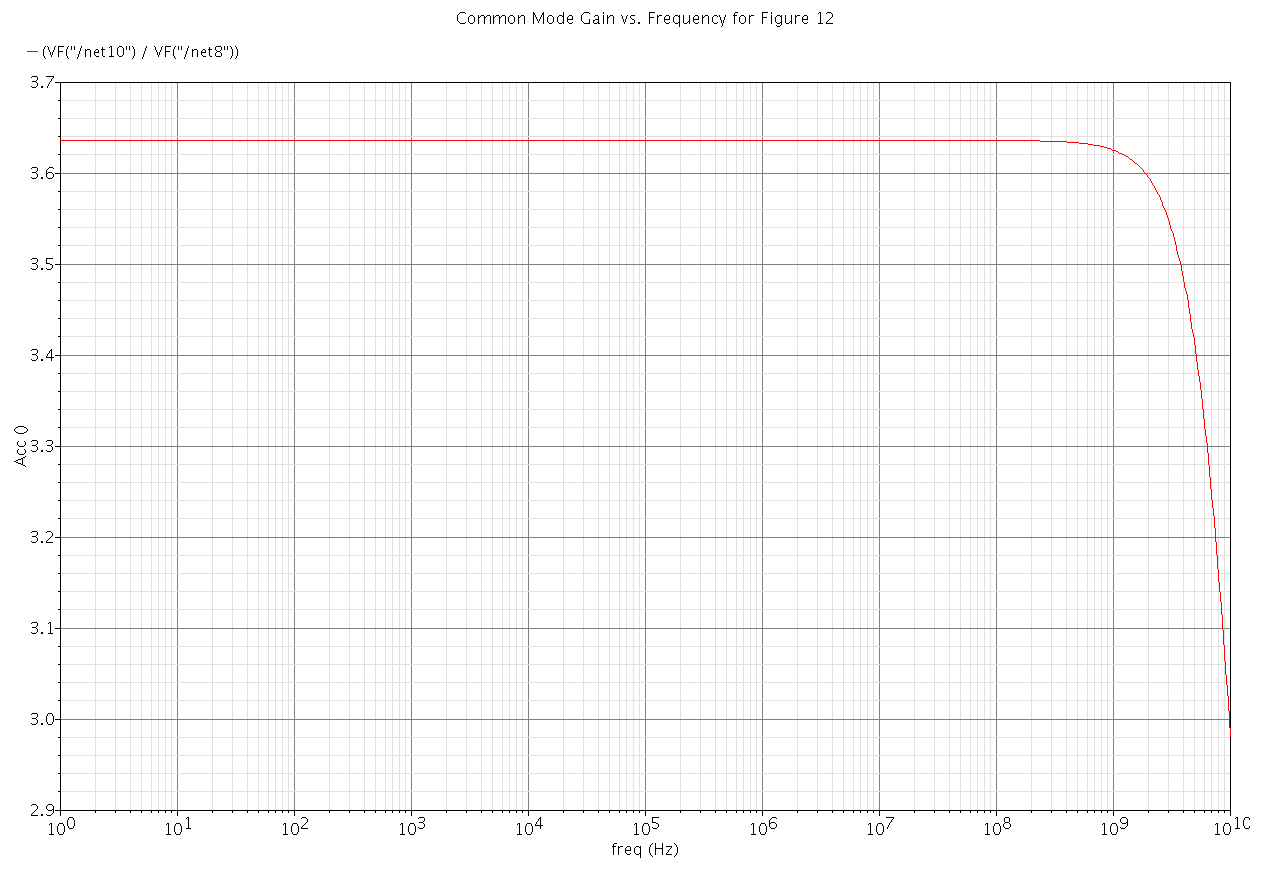
\includegraphics[width=6in]{p3_3b}
\caption{Common Mode Gain vs. Frequency for Figure 12}
\label{3_3b_gain}
\end{figure}

\begin{figure}[H]
\centering
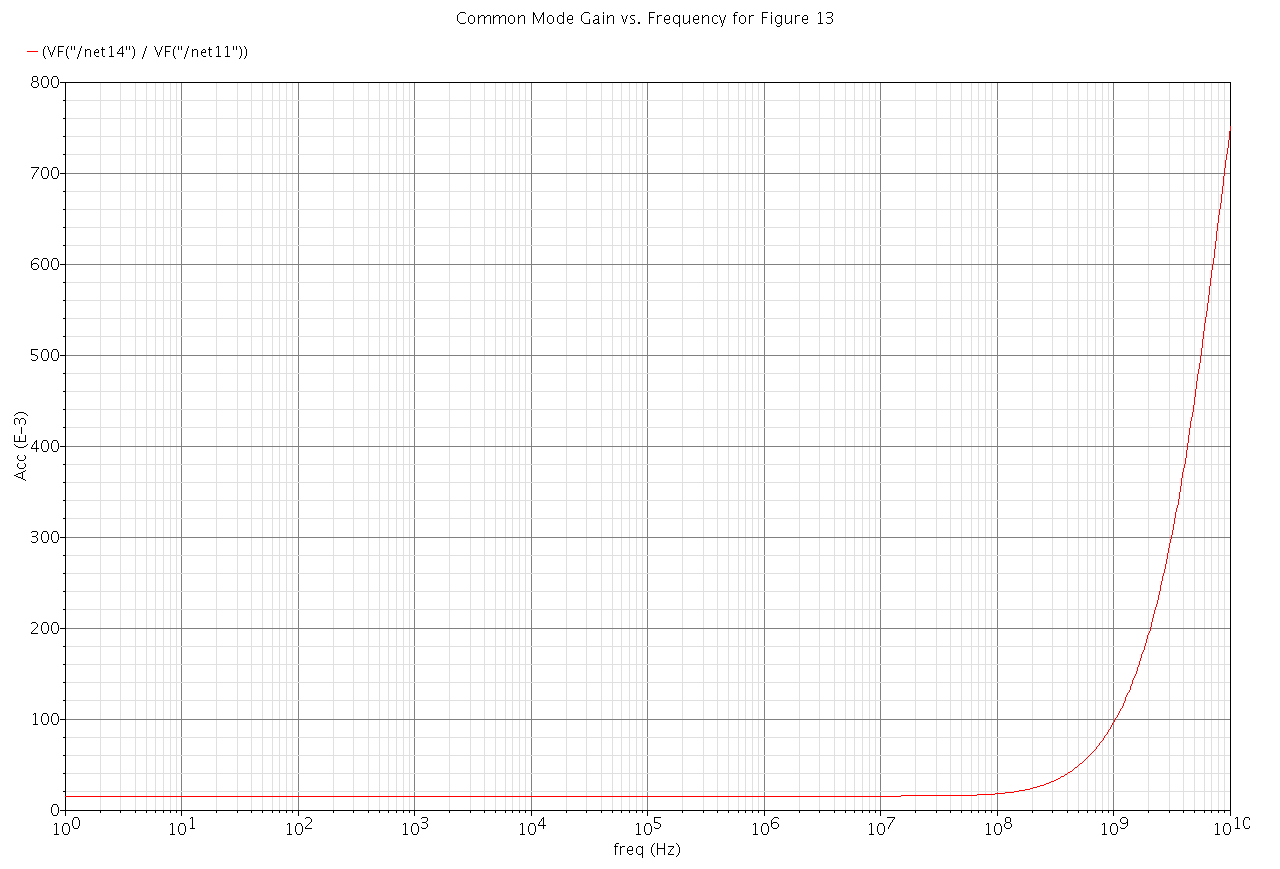
\includegraphics[width=6in]{p3_3c}
\caption{Common Mode Gain vs. Frequency for Figure 13}
\label{3_3c_gain}
\end{figure}

\subsection{}

\begin{figure}[H]
\centering
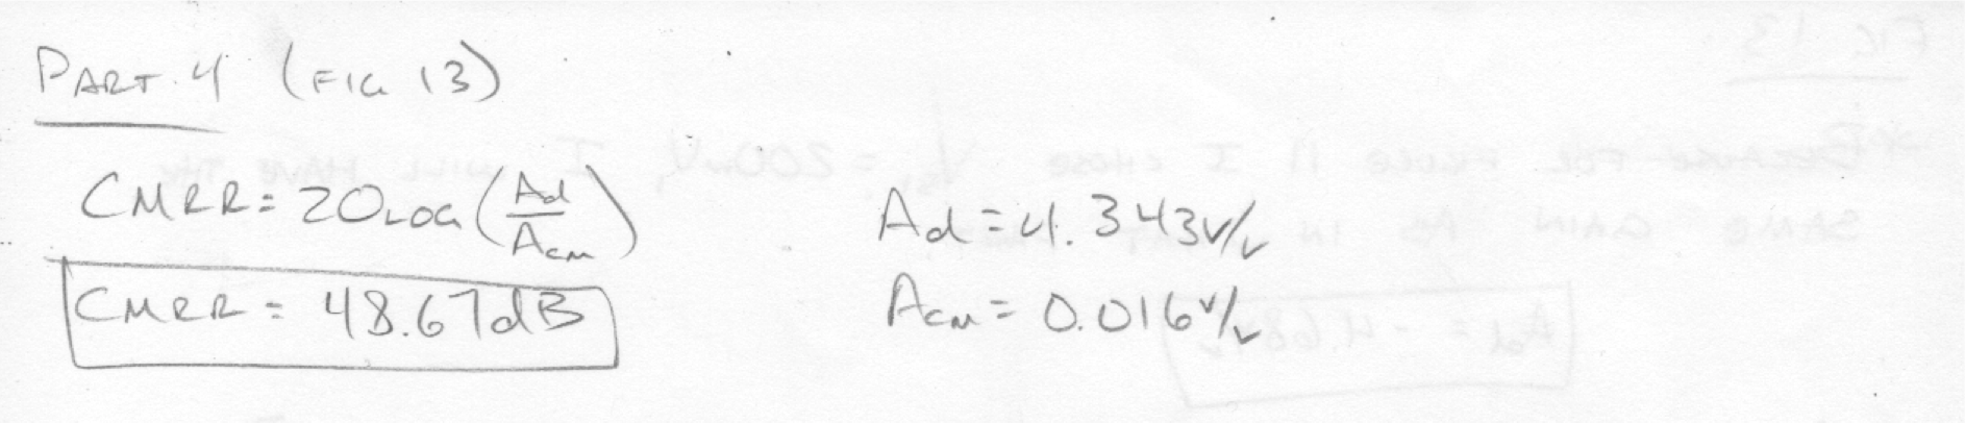
\includegraphics[width=6in]{1_11a}
\caption{Hand-Written Work for Problem 3.4}
\label{3_4}
\end{figure}
\newpage

\subsection{}
CMRR can be increased by increasing the resistance of the current source ($R_{SS}$). To do this, we utilize the cascade current mirror as developed earlier in the problem set.

\begin{figure}[H]
\centering
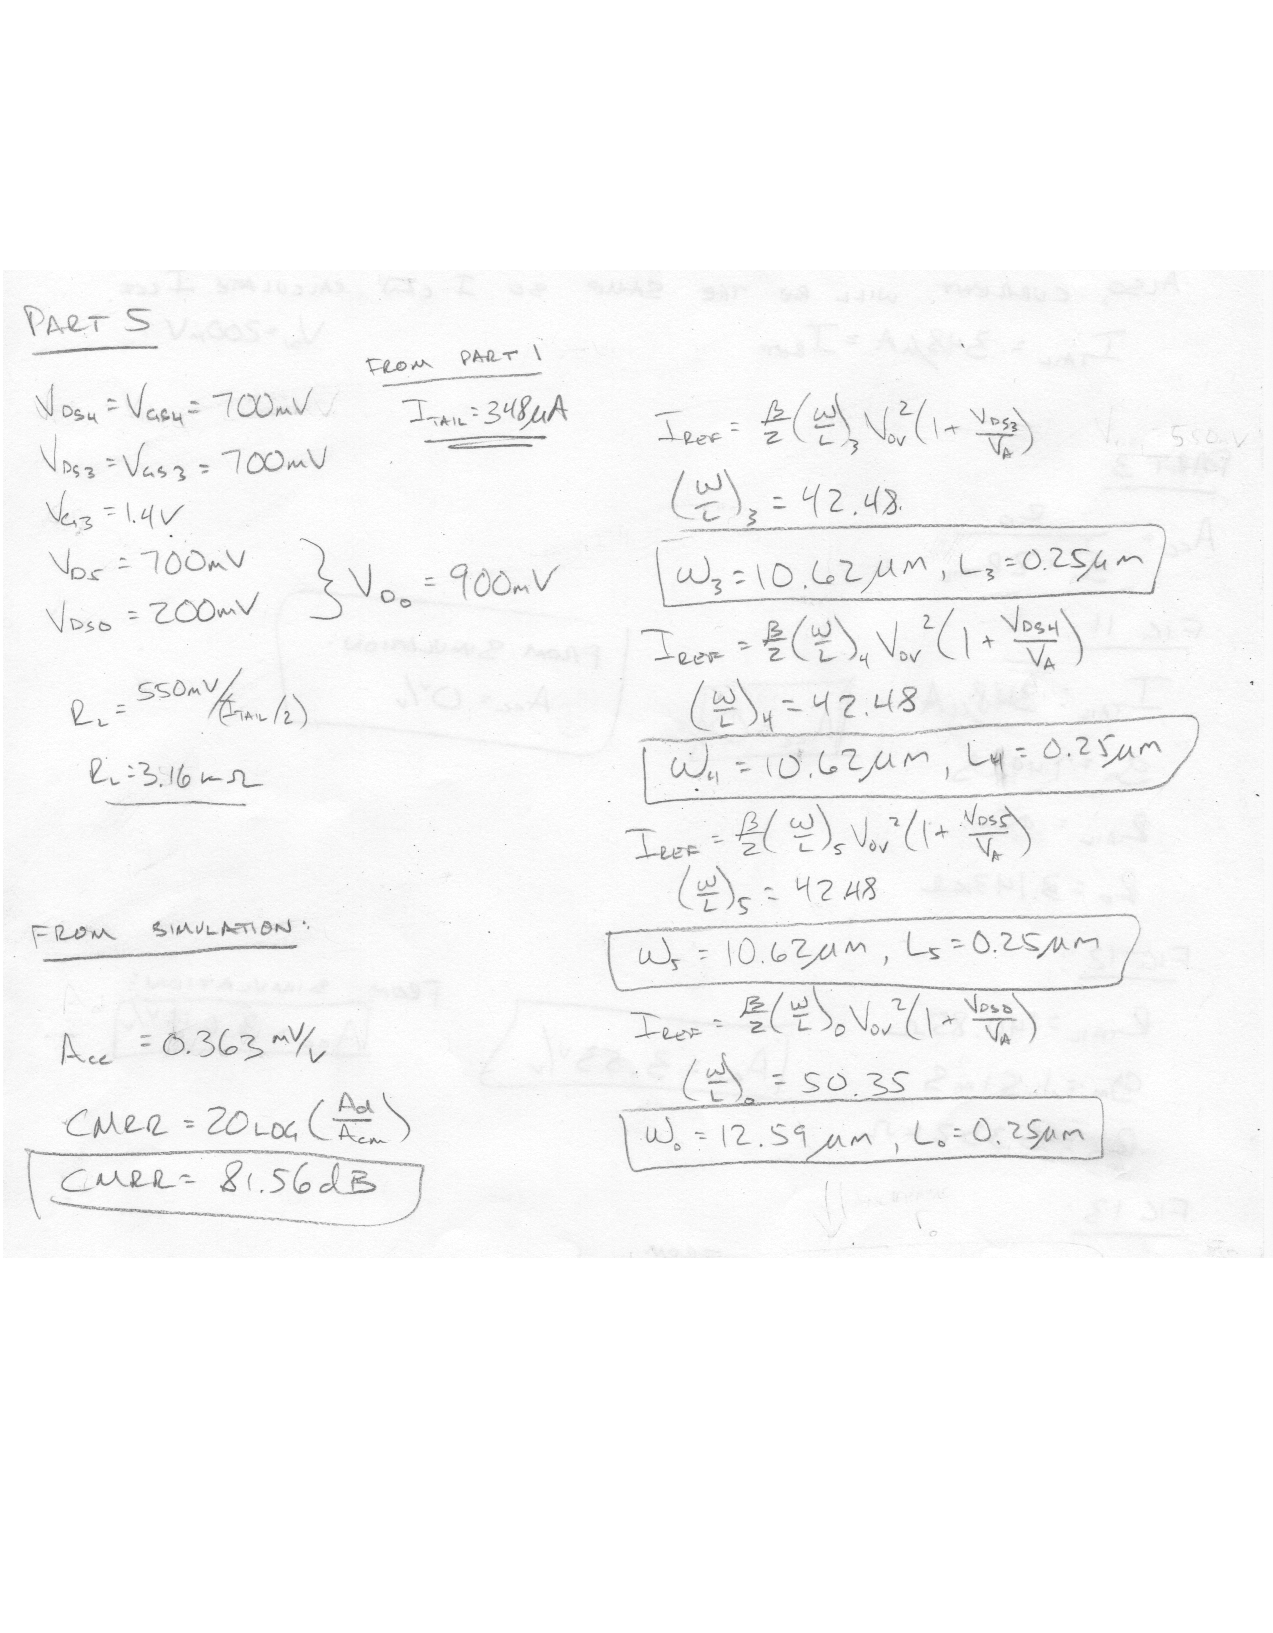
\includegraphics[width=6in]{1_11}
\caption{Hand-Written Work for Problem 3.5}
\label{3_5}
\end{figure}

\begin{figure}[H]
\centering
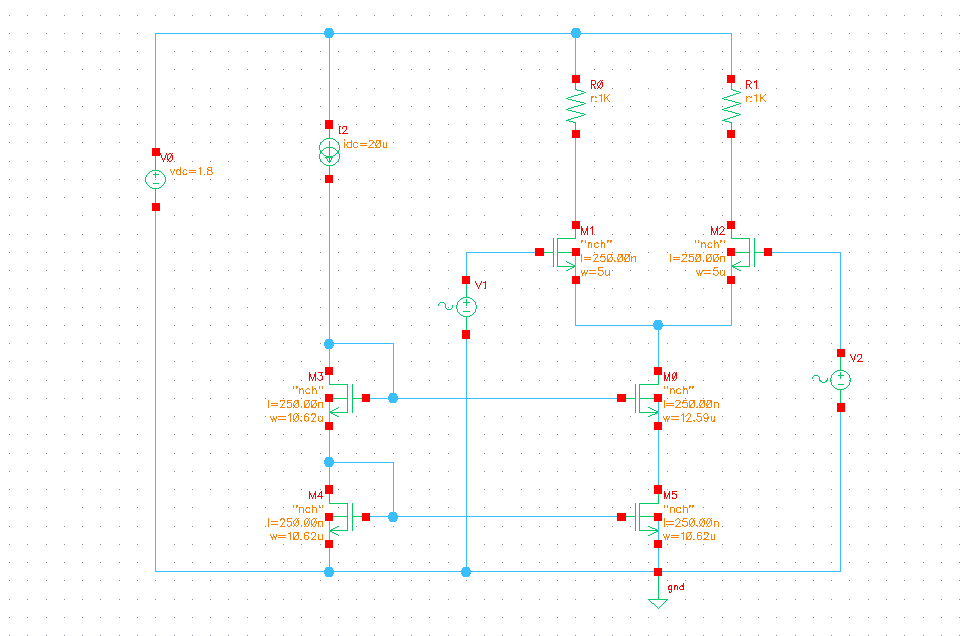
\includegraphics[width=6in]{p3_5_schem}
\caption{Schematic to Improve CMRR of the Differential Amplifier}
\label{3_5_schem}
\end{figure}


\end{document}
